%%%%%%%%%%%%%%%%%%%%%%%%%%%%%%%%%%%%%%%%%%%%%%%%%%%%%%%%%%%%%%%%%%%%%%%%%%%%%%%%%%
\begin{frame}[fragile]\frametitle{}
\begin{center}
{\Large Modern RL}
\end{center}
\end{frame}

%%%%%%%%%%%%%%%%%%%%%%%%%%%%%%%%%%%%%%%%%%%%%%%%%%%%%%%%%%%%%%%%%%%%%%%%%%%%%%%%%%
\begin{frame}[fragile]\frametitle{}
\begin{center}
{\Large Curiosity}
\end{center}
\end{frame}

%%%%%%%%%%%%%%%%%%%%%%%%%%%%%%%%%%%%%%%%%%%%%%%%%%%%%%%%%%%%%%%%%%%%%%%%%%%%%%%%%%
\begin{frame}[fragile]\frametitle{Reinforce (Problems)}

Two Major Problems in Modern RL

\begin{itemize}
\item Sparse rewards or non-existing rewards problem: that is, most rewards do not contain information, and hence are set to zero. However, as rewards act as feedback for RL agents, if they don’t receive any, their knowledge of which action is appropriate (or not) cannot change. For instance, in Vizdoom “DoomMyWayHome,” your agent is only rewarded if it finds the vest. However, the vest is far away from your starting point, so most of your rewards will be zero.
\item Extrinsic reward function is handmade — that is, in each environment, a human has to implement a reward function. But how we can scale that in big and complex environments?
\item Therefore, a solution to these problems is to develop a reward function that is intrinsic to the agent, i.e., generated by the agent itself. 
\end{itemize}

{\tiny (Ref: Curiosity-Driven Learning through Next State Prediction - Thomas Simonini)}

\end{frame}

%%%%%%%%%%%%%%%%%%%%%%%%%%%%%%%%%%%%%%%%%%%%%%%%%%%%%%%%%%%%%%%%%%%%%%%%%%%%%%%%%%
\begin{frame}[fragile]\frametitle{Curiosity}
Curiosity-Driven Learning through Next State Prediction

% \begin{center}
% 
\includegraphics[width=0.4\linewidth,keepaspectratio]{rl59}
% \end{center}

\begin{itemize}
\item MThe idea of curiosity-driven learning is to build a reward function that is intrinsic to the agent (that is generated by the agent itself). In this sense, the agent will act as a self-learner since it will be the student, but also its own feedback master.
\item This intrinsic reward mechanism is known as curiosity because it explores states that are novel/unfamiliar. In order to achieve that, our agent will receive a high reward when exploring new trajectories.
\item This reward design is based on how human plays — some suppose we have an intrinsic desire to explore environments and discover new things! There are different ways to calculate this intrinsic reward, and we’ll focus on this article on curiosity through next-state prediction.
\end{itemize}

{\tiny (Ref: Curiosity-Driven Learning through Next State Prediction - Thomas Simonini)}


\end{frame}


%%%%%%%%%%%%%%%%%%%%%%%%%%%%%%%%%%%%%%%%%%%%%%%%%%%%%%%%%%%%%%%%%%%%%%%%%%%%%%%%%%
\begin{frame}[fragile]\frametitle{Super Mario Bros}
Curiosity-Driven Learning through Next State Prediction

\begin{center}
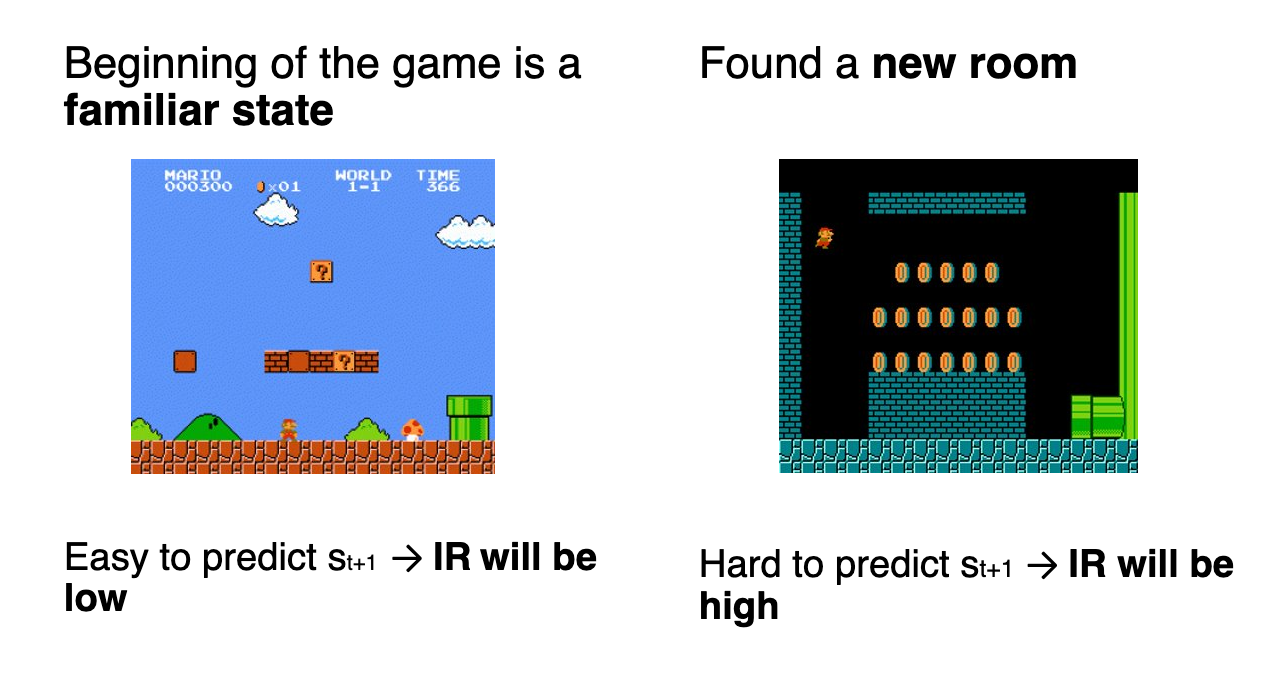
\includegraphics[width=0.6\linewidth,keepaspectratio]{rl130}
\end{center}

\begin{itemize}
\item If you spend a lot of time in the beginning of the game (which is not new), the agent will be able to accurately predict what the next state will be, so the reward will be low.
\item  On the other hand, if you discover a new room, our agent will be very bad in predicting the next state, so the agent will be pushed to explore this room.
\end{itemize}

{\tiny (Ref: Curiosity-Driven Learning through Next State Prediction - Thomas Simonini)}


\end{frame}

%%%%%%%%%%%%%%%%%%%%%%%%%%%%%%%%%%%%%%%%%%%%%%%%%%%%%%%%%%%%%%%%%%%%%%%%%%%%%%%%%%
\begin{frame}[fragile]\frametitle{Super Mario Bros}


\begin{itemize}
\item Consequently, measuring error requires building a model of environmental dynamics that predicts the next state given the current state and the action. The question that we can ask here is: how we can calculate this error?
\item But we can’t predict $s_{t+1}$ by predicting the next frame as we usually do. Why?
\item First, because it’s hard to build a model that is able to predict high-dimension continuous state space, such as an image. It’s hard to predict the pixels directly, but now imagine you’re in Doom, and you move left — you need to predict 248*248 = 61504 pixels!
\end{itemize}

{\tiny (Ref: Curiosity-Driven Learning through Next State Prediction - Thomas Simonini)}


\end{frame}

%%%%%%%%%%%%%%%%%%%%%%%%%%%%%%%%%%%%%%%%%%%%%%%%%%%%%%%%%%%%%%%%%%%%%%%%%%%%%%%%%%
\begin{frame}[fragile]\frametitle{Super Mario Bros}


It means that in order to generate curiosity, we can’t predict the pixels directly and need to use a better feature representation by projecting the raw pixels space into a feature space that will hopefully only keep the relevant information elements that can be leveraged by our agent.


\begin{center}
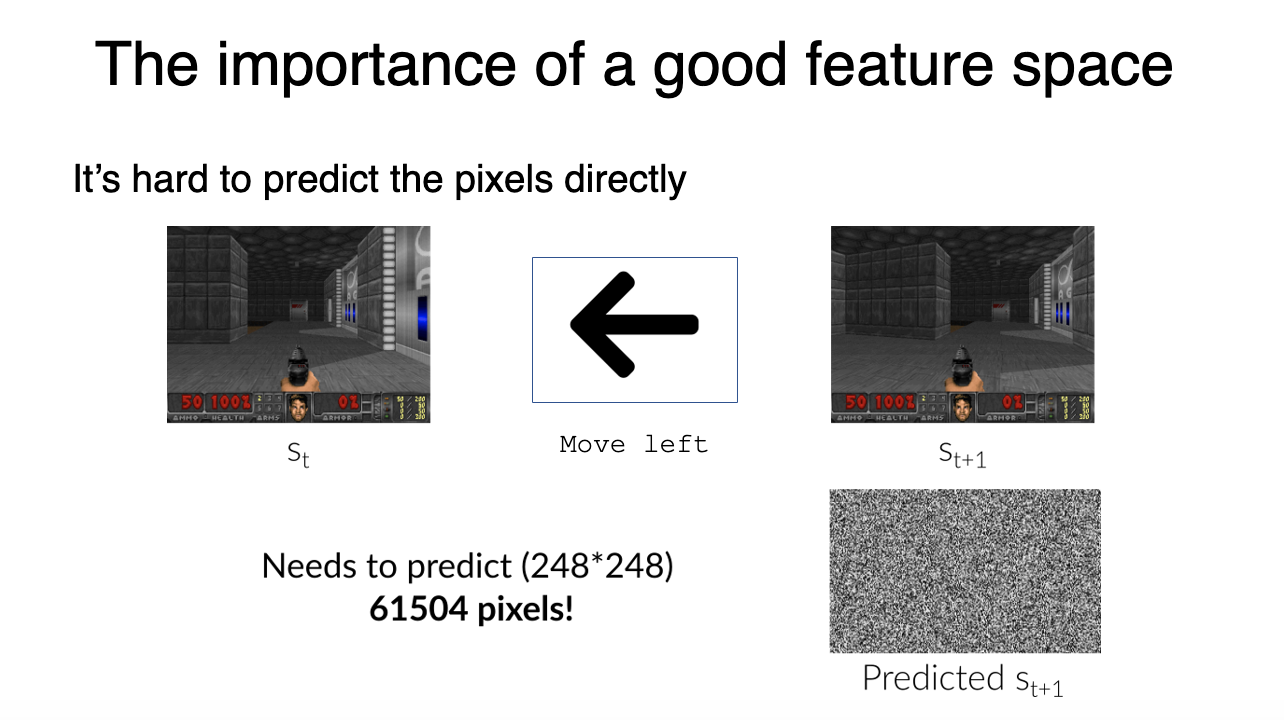
\includegraphics[width=0.8\linewidth,keepaspectratio]{rl131}
\end{center}

{\tiny (Ref: Curiosity-Driven Learning through Next State Prediction - Thomas Simonini)}


\end{frame}

%%%%%%%%%%%%%%%%%%%%%%%%%%%%%%%%%%%%%%%%%%%%%%%%%%%%%%%%%%%%%%%%%%%%%%%%%%%%%%%%%%
\begin{frame}[fragile]\frametitle{Super Mario Bros}

Three rules are defined in the original paper for a good representation feature space:

\begin{itemize}
\item Model things that can be controlled by the agent.
\item Model things that can’t be controlled by the agent but can affect the agent.
\item Don’t model things that are not controlled by the agent and have no effect on it.
\end{itemize}

The second reason we can’t predict $s_{t+1}$ by predicting the next frame as we usually do? It might just not be the right thing to do:

{\tiny (Ref: Curiosity-Driven Learning through Next State Prediction - Thomas Simonini)}


\end{frame}

%%%%%%%%%%%%%%%%%%%%%%%%%%%%%%%%%%%%%%%%%%%%%%%%%%%%%%%%%%%%%%%%%%%%%%%%%%%%%%%%%%
\begin{frame}[fragile]\frametitle{Car}



\begin{itemize}
\item Imagine you need to study the movement of the tree leaves in a breeze. First of all, it’s already hard enough to model breeze, so predicting the pixel location of each leaves at each time step is even harder.
\item So instead of making predictions in the raw sensory space (pixels), we need to transform the raw sensory input (array of pixels) into a feature space with only relevant information.
\item Let’s take this example: your agent is a self driving car. If we want to create a good feature representation, we need to model:
\end{itemize}

\begin{center}
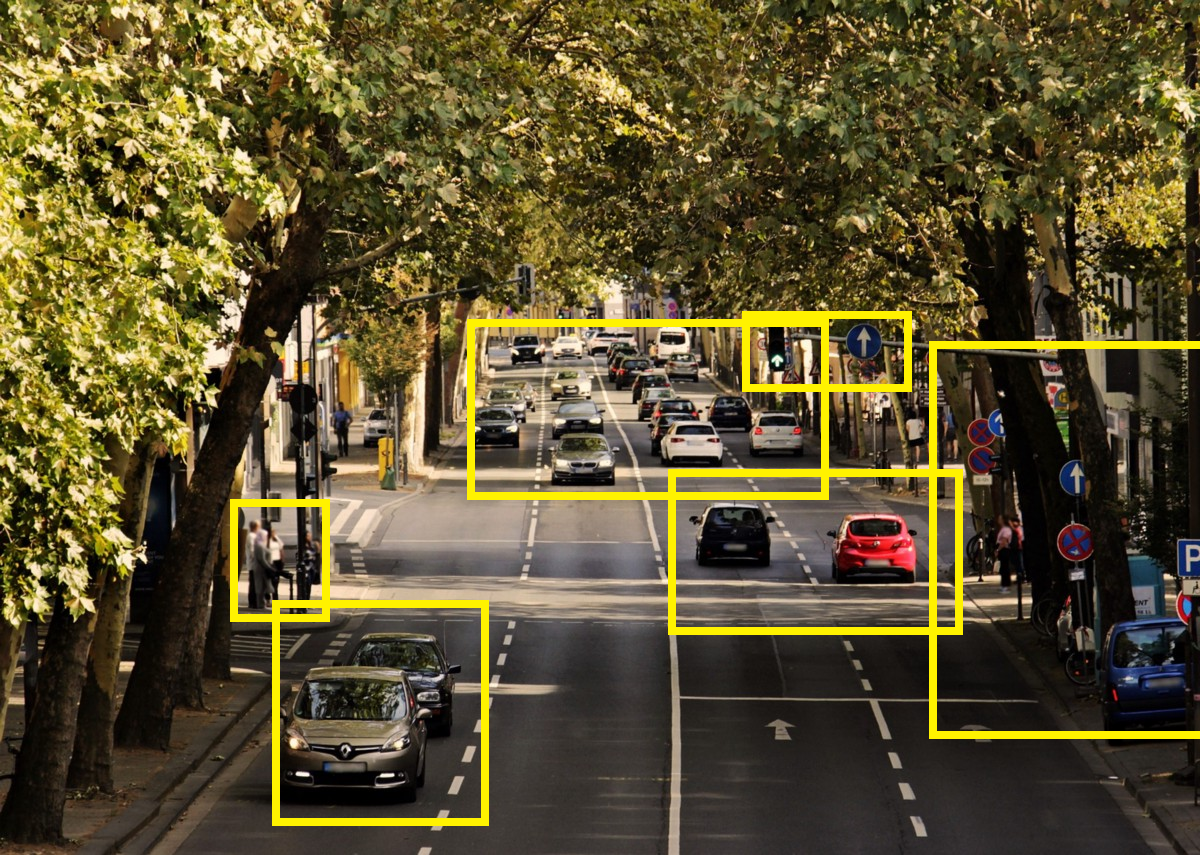
\includegraphics[width=0.4\linewidth,keepaspectratio]{rl132}
\end{center}


{\tiny (Ref: Curiosity-Driven Learning through Next State Prediction - Thomas Simonini)}


\end{frame}

%%%%%%%%%%%%%%%%%%%%%%%%%%%%%%%%%%%%%%%%%%%%%%%%%%%%%%%%%%%%%%%%%%%%%%%%%%%%%%%%%%
\begin{frame}[fragile]\frametitle{Feature Representation}

A good feature representation would be our car (controlled by our agent) and the other cars (we can’t control it, but that can affect the agent), but we don’t need to model the leaves (it doesn’t affect the agent, and we can’t control it). By only keeping this information, we will have a feature representation with less noise.

The desired embedding space should:

\begin{itemize}
\item Be compact in terms of dimensional (remove irrelevant parts of the observation space).
\item Preserve sufficient information about the observation.
\item Be stable, because non-stationary rewards (rewards that decrease through time since curiosity decreases through time) make it difficult for reinforcement agents to learn.
\end{itemize}

In order to calculate the predicted next state and the real feature representation of the next state, we can use an Intrinsic Curiosity Module (ICM).

{\tiny (Ref: Curiosity-Driven Learning through Next State Prediction - Thomas Simonini)}


\end{frame}

%%%%%%%%%%%%%%%%%%%%%%%%%%%%%%%%%%%%%%%%%%%%%%%%%%%%%%%%%%%%%%%%%%%%%%%%%%%%%%%%%%
\begin{frame}[fragile]\frametitle{ICM Module}

The ICM Module is the system that helps us to generate curiosity. It’s composed of two neural networks; each of them has an important task.

\begin{center}
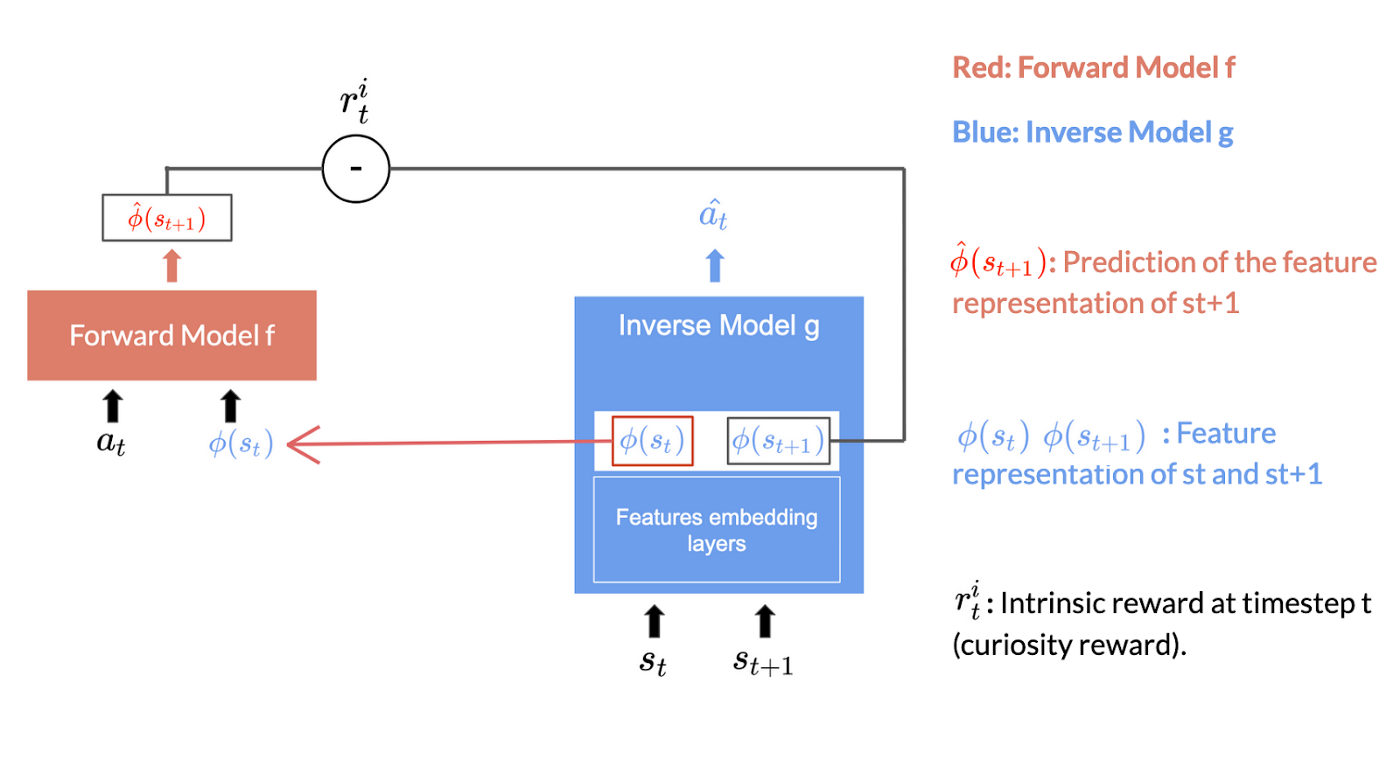
\includegraphics[width=\linewidth,keepaspectratio]{rl133}
\end{center}


{\tiny (Ref: Curiosity-Driven Learning through Next State Prediction - Thomas Simonini)}


\end{frame}

%%%%%%%%%%%%%%%%%%%%%%%%%%%%%%%%%%%%%%%%%%%%%%%%%%%%%%%%%%%%%%%%%%%%%%%%%%%%%%%%%%
\begin{frame}[fragile]\frametitle{The Inverse Model}

The Inverse Model (g), aims at predicting the action $a(t)$, and in doing so, it learns an internal feature representation of the state and next state, denoted by $\phi(s(t))$ and $\phi(s(t+1))$.
\begin{center}
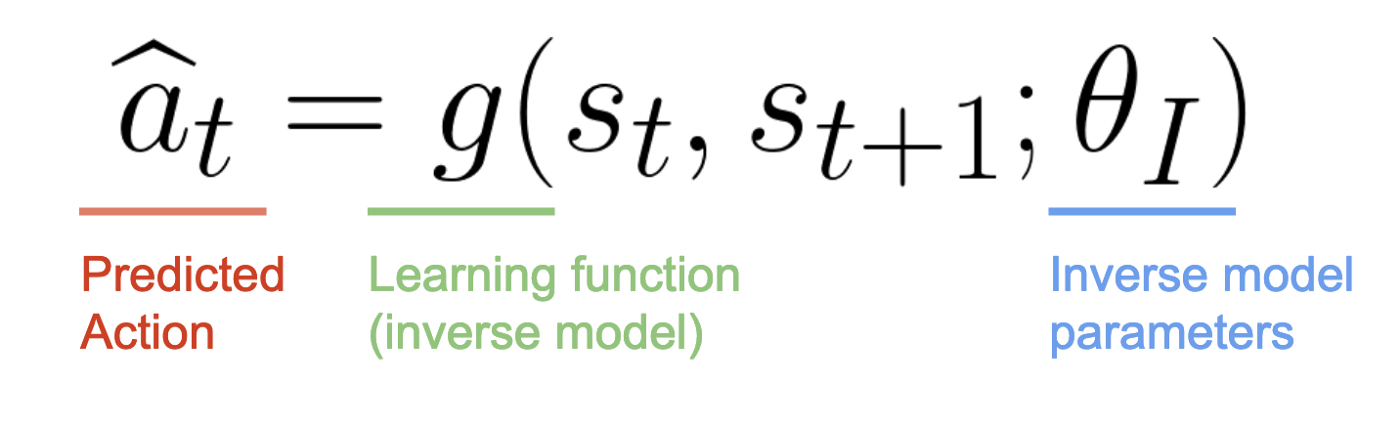
\includegraphics[width=0.6\linewidth,keepaspectratio]{rl134}
\end{center}

Since this neural network is only used to predict the action, it has no incentive to represent within its feature embedding space the factors of variation in an environment that does not affect the agent itself.


{\tiny (Ref: Curiosity-Driven Learning through Next State Prediction - Thomas Simonini)}


\end{frame}

%%%%%%%%%%%%%%%%%%%%%%%%%%%%%%%%%%%%%%%%%%%%%%%%%%%%%%%%%%%%%%%%%%%%%%%%%%%%%%%%%%
\begin{frame}[fragile]\frametitle{The Inverse Model}

Lastly, the inverse model loss is given by the cross entropy between our predicted action â(t) and the real action a(t):


\begin{center}
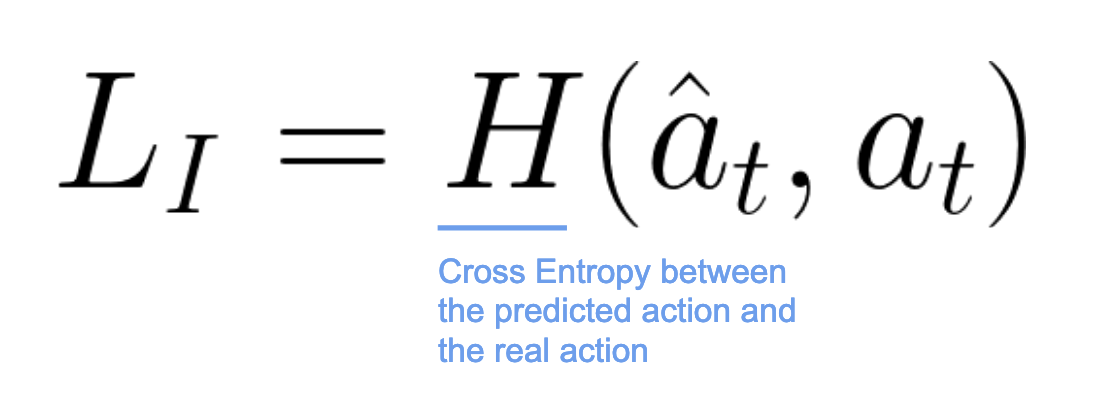
\includegraphics[width=0.4\linewidth,keepaspectratio]{rl135}
\end{center}



{\tiny (Ref: Curiosity-Driven Learning through Next State Prediction - Thomas Simonini)}


\end{frame}

%%%%%%%%%%%%%%%%%%%%%%%%%%%%%%%%%%%%%%%%%%%%%%%%%%%%%%%%%%%%%%%%%%%%%%%%%%%%%%%%%%
\begin{frame}[fragile]\frametitle{The Forward model}

The Forward Model (f), predicts the feature representation of next state $\phi(s(t+1))$ given $\phi(s(t))$ and $a(t)$.

\begin{center}
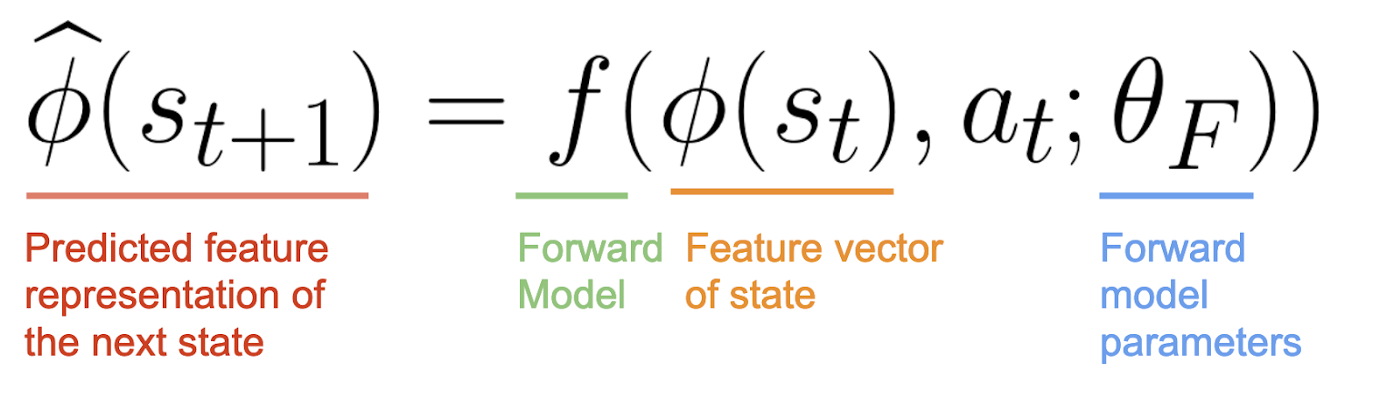
\includegraphics[width=0.6\linewidth,keepaspectratio]{rl136}
\end{center}

Consequently, curiosity will be a real number, i.e., the L2 normed difference between our predicted feature vector of the next state

Finally, the overall optimization problem of this module is a composition of Inverse Loss and Forward Loss.

And we provide the prediction error of the forward dynamics model to the agent as an intrinsic reward to encourage its curiosity.

{\tiny (Ref: Curiosity-Driven Learning through Next State Prediction - Thomas Simonini)}


\end{frame}


%%%%%%%%%%%%%%%%%%%%%%%%%%%%%%%%%%%%%%%%%%%%%%%%%%%%%%%%%%%%%%%%%%%%%%%%%%%%%%%%%%
\begin{frame}[fragile]\frametitle{}
\begin{center}
{\Large Advantage Actor Critic (A2C)}
\end{center}

{\tiny (Ref: Advantage Actor Critic (A2C)  https://huggingface.co/blog/deep-rl-a2c)}

\end{frame}

%%%%%%%%%%%%%%%%%%%%%%%%%%%%%%%%%%%%%%%%%%%%%%%%%%%%%%%%%%%%%%%%%%%%%%%%%%%%%%%%%%
\begin{frame}[fragile]\frametitle{Background}


\begin{itemize}
\item In Policy-Based methods, we aim to optimize the policy directly without using a value function. More precisely, Reinforce is part of a subclass of Policy-Based Methods called Policy-Gradient methods. This subclass optimizes the policy directly by estimating the weights of the optimal policy using Gradient Ascent.
\item 
We saw that Reinforce worked well. However, because we use Monte-Carlo sampling to estimate return (we use an entire episode to calculate the return), we have significant variance in policy gradient estimation.
\item 
Remember that the policy gradient estimation is the direction of the steepest increase in return. Aka, how to update our policy weights so that actions that lead to good returns have a higher probability of being taken. The Monte Carlo variance, which we will further study in this unit, leads to slower training since we need a lot of samples to mitigate it.
\end{itemize}


\end{frame}

%%%%%%%%%%%%%%%%%%%%%%%%%%%%%%%%%%%%%%%%%%%%%%%%%%%%%%%%%%%%%%%%%%%%%%%%%%%%%%%%%%
\begin{frame}[fragile]\frametitle{The Problem of Variance in Reinforce}


\begin{itemize}
\item In Reinforce, we want to increase the probability of actions in a trajectory proportional to how high the return is.
\item If the return is high, we will push up the probabilities of the (state, action) combinations.
\item Else, if the return is low, it will push down the probabilities of the (state, action) combinations.
\end{itemize}

\begin{center}
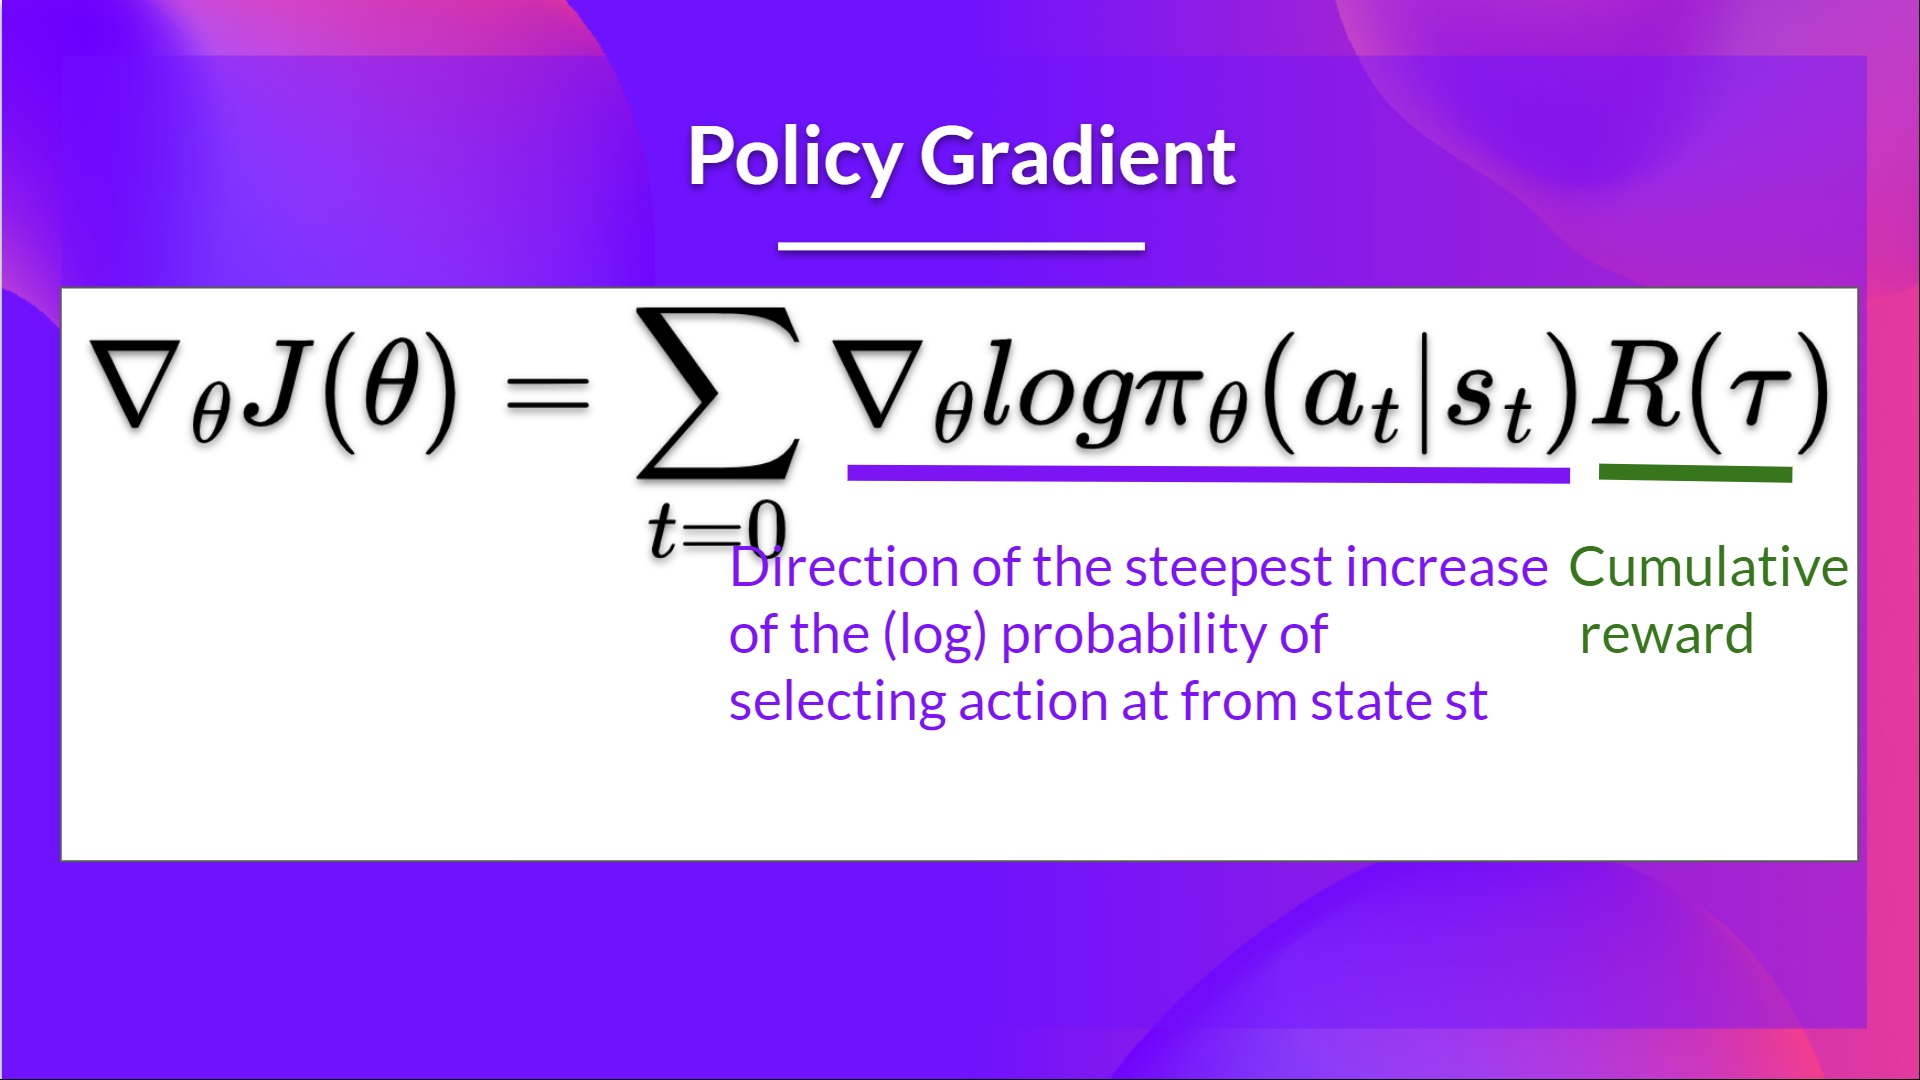
\includegraphics[width=0.6\linewidth,keepaspectratio]{rl137}
\end{center}

\end{frame}

%%%%%%%%%%%%%%%%%%%%%%%%%%%%%%%%%%%%%%%%%%%%%%%%%%%%%%%%%%%%%%%%%%%%%%%%%%%%%%%%%%
\begin{frame}[fragile]\frametitle{The Problem of Variance in Reinforce}


\begin{itemize}
\item This return $R(\tau)$ is calculated using a Monte-Carlo sampling. Indeed, we collect a trajectory and calculate the discounted return, and use this score to increase or decrease the probability of every action taken in that trajectory. If the return is good, all actions will be “reinforced” by increasing their likelihood of being taken. $R(\tau) = R_{t+1} + \gamma R_{t+2} + \gamma^2 R_{t+3} + \ldots$
\item The advantage of this method is that it’s unbiased. Since we’re not estimating the return, we use only the true return we obtain.

\end{itemize}



\end{frame}

%%%%%%%%%%%%%%%%%%%%%%%%%%%%%%%%%%%%%%%%%%%%%%%%%%%%%%%%%%%%%%%%%%%%%%%%%%%%%%%%%%
\begin{frame}[fragile]\frametitle{The Problem of Variance in Reinforce}


\begin{itemize}
\item But the problem is that the variance is high, since trajectories can lead to different returns due to stochasticity of the environment (random events during episode) and stochasticity of the policy. Consequently, the same starting state can lead to very different returns. 
\item Because of this, the return starting at the same state can vary significantly across episodes.
\end{itemize}

\begin{center}
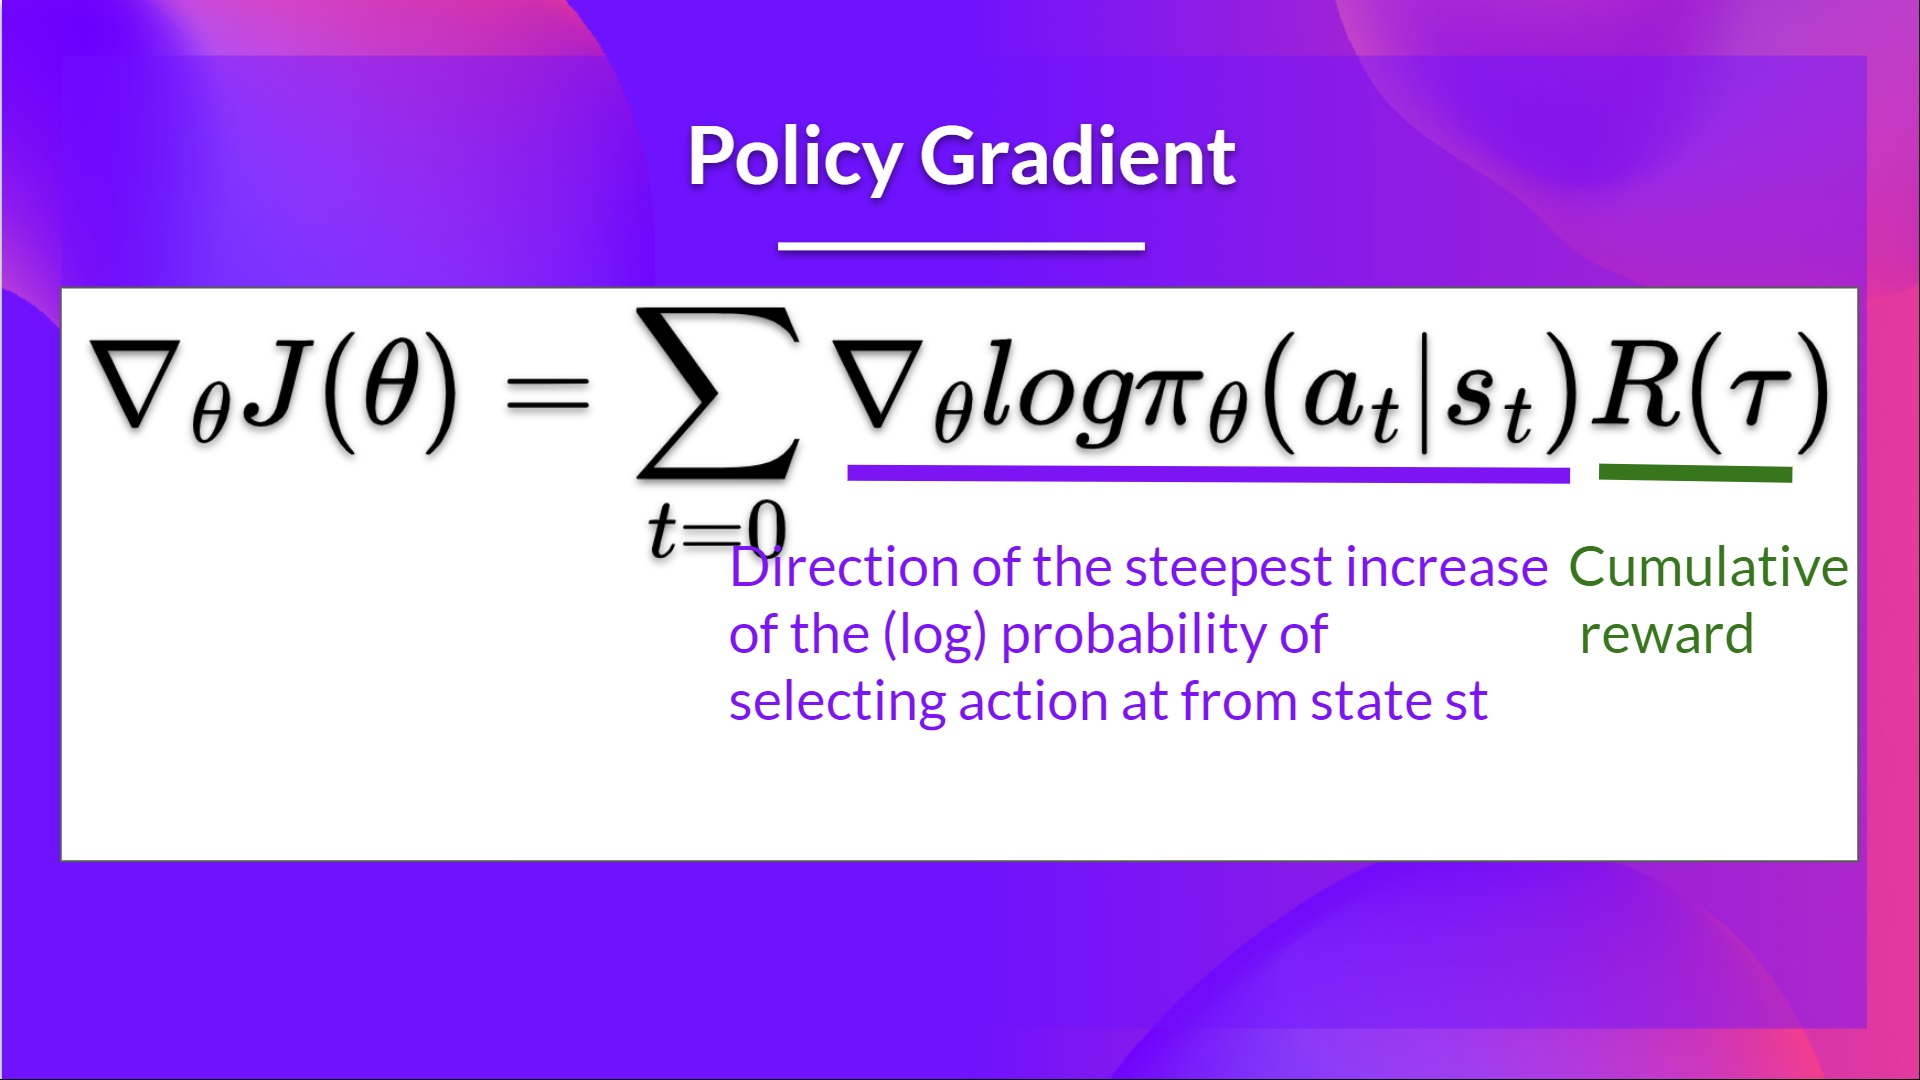
\includegraphics[width=0.6\linewidth,keepaspectratio]{rl137}
\end{center}


\end{frame}



%%%%%%%%%%%%%%%%%%%%%%%%%%%%%%%%%%%%%%%%%%%%%%%%%%%%%%%%%%%%%%%%%%%%%%%%%%%%%%%%%%
\begin{frame}[fragile]\frametitle{The Problem of Variance in Reinforce}


\begin{itemize}
\item The solution is to mitigate the variance by using a large number of trajectories, hoping that the variance introduced in any one trajectory will be reduced in aggregate and provide a "true" estimation of the return.
\item 
However, increasing the batch size significantly reduces sample efficiency. So we need to find additional mechanisms to reduce the variance.
\end{itemize}


\end{frame}


%%%%%%%%%%%%%%%%%%%%%%%%%%%%%%%%%%%%%%%%%%%%%%%%%%%%%%%%%%%%%%%%%%%%%%%%%%%%%%%%%%
\begin{frame}[fragile]\frametitle{Introduction}


\begin{itemize}
\item Actor-Critic methods, a hybrid architecture combining a value-based and policy-based methods that help to stabilize the training by reducing the variance
\item An Actor that controls how our agent behaves (policy-based method)
\item A Critic that measures how good the action taken is (value-based method
\end{itemize}


\end{frame}

%%%%%%%%%%%%%%%%%%%%%%%%%%%%%%%%%%%%%%%%%%%%%%%%%%%%%%%%%%%%%%%%%%%%%%%%%%%%%%%%%%
\begin{frame}[fragile]\frametitle{Reducing variance with Actor-Critic methods}


\begin{itemize}
\item The solution to reducing the variance of Reinforce algorithm and training our agent faster and better is to use a combination of policy-based and value-based methods: the Actor-Critic method.
\item 
To understand the Actor-Critic, imagine you play a video game. You can play with a friend that will provide you some feedback. You’re the Actor, and your friend is the Critic.
\end{itemize}

\begin{center}

\includegraphics[width=0.6\linewidth,keepaspectratio]{rl139}
\end{center}

\end{frame}

%%%%%%%%%%%%%%%%%%%%%%%%%%%%%%%%%%%%%%%%%%%%%%%%%%%%%%%%%%%%%%%%%%%%%%%%%%%%%%%%%%
\begin{frame}[fragile]\frametitle{Reducing variance with Actor-Critic methods}
\begin{itemize}
\item You don’t know how to play at the beginning, so you try some actions randomly. The Critic observes your action and provides feedback.
\item Learning from this feedback, you’ll update your policy and be better at playing that game.
\item On the other hand, your friend (Critic) will also update their way to provide feedback so it can be better next time.
\item We learn two function approximations:
\begin{itemize}
\item A policy that controls how our agent acts: $\pi_{\theta}(s,a)$
\item A value function to assist the policy update by measuring how good the action taken is: $\hat{q}_{w}(s,a)$
\end{itemize}
\end{itemize}
\end{frame}

%%%%%%%%%%%%%%%%%%%%%%%%%%%%%%%%%%%%%%%%%%%%%%%%%%%%%%%%%%%%%%%%%%%%%%%%%%%%%%%%%%
\begin{frame}[fragile]\frametitle{The Actor-Critic Process}
Let's see the training process to understand how Actor and Critic are optimized

\begin{itemize}
\item At each timestep, $t$, we get the current state $S_t$ from the environment and pass it as input through our Actor and Critic.
\item Our Policy takes the state and outputs an action $A_t$.
\end{itemize}

\begin{center}
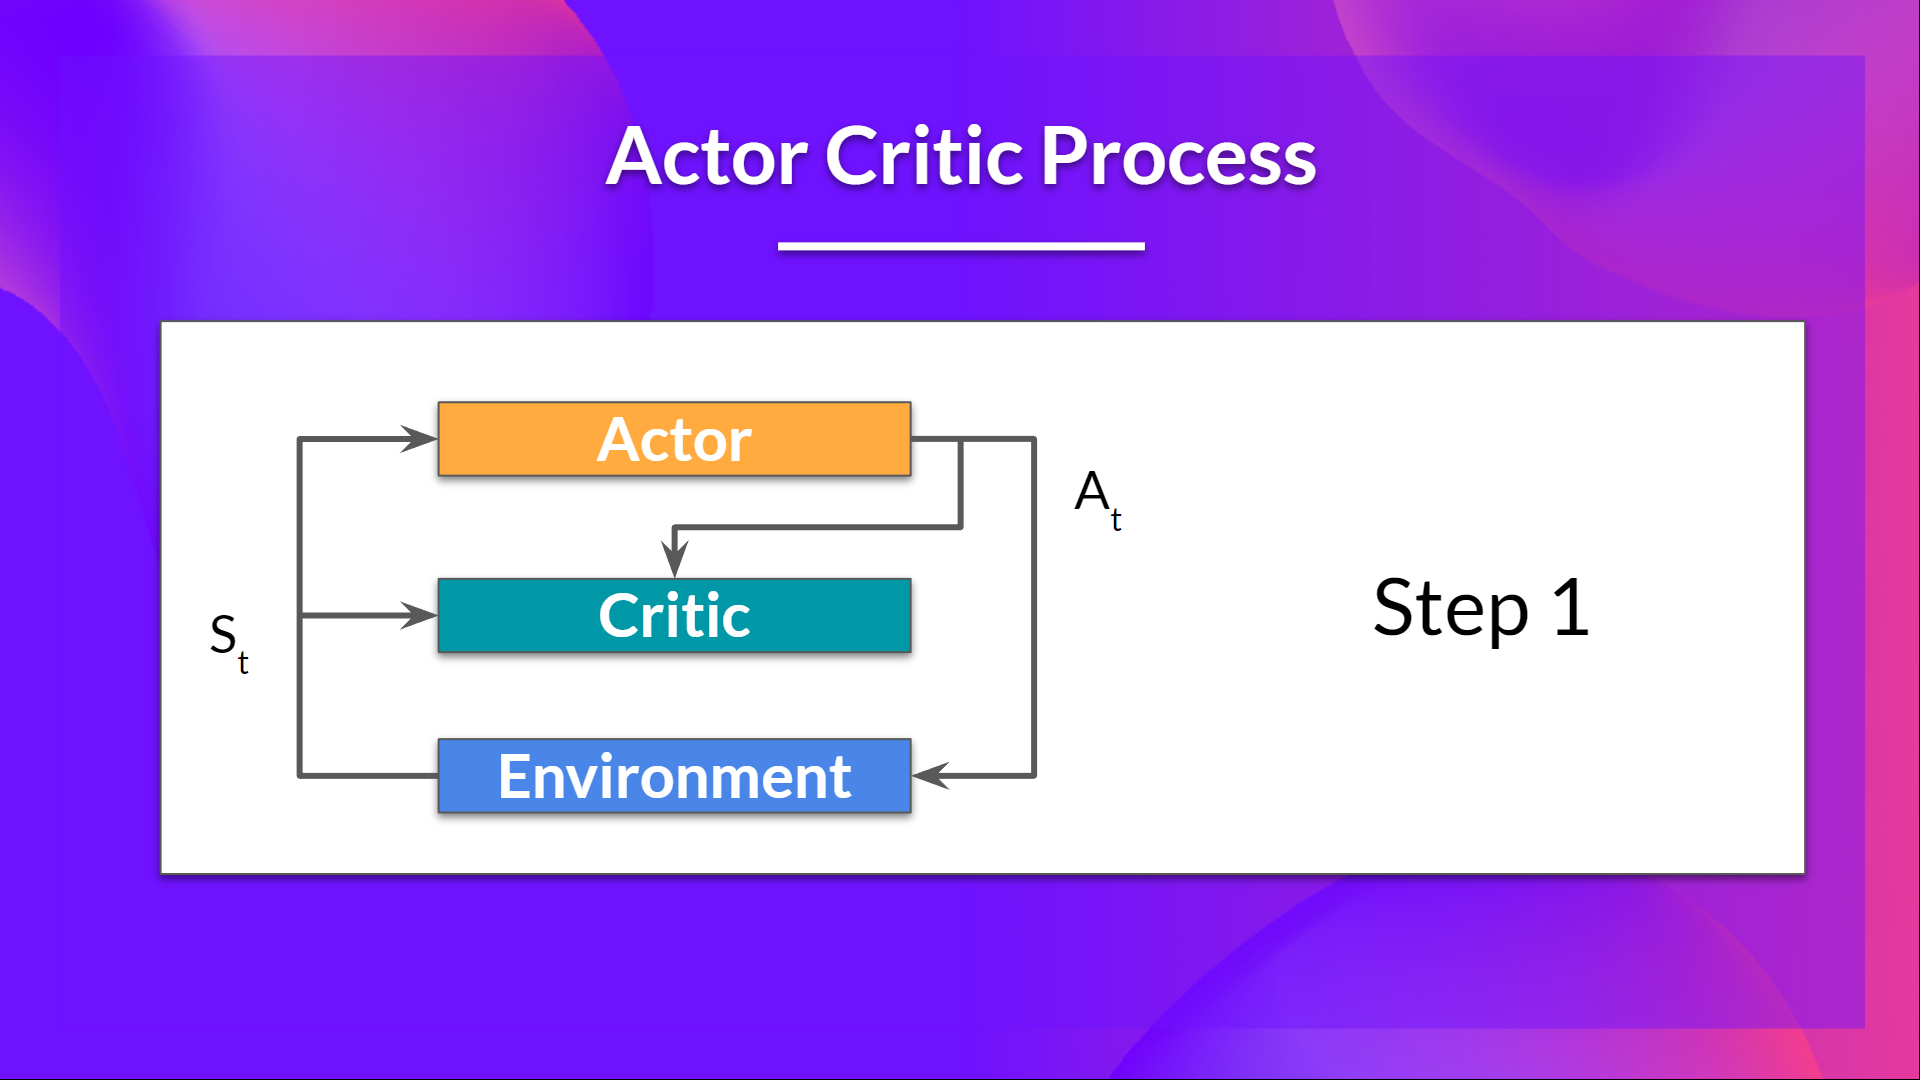
\includegraphics[width=0.6\linewidth,keepaspectratio]{rl140}
\end{center}
\end{frame}

%%%%%%%%%%%%%%%%%%%%%%%%%%%%%%%%%%%%%%%%%%%%%%%%%%%%%%%%%%%%%%%%%%%%%%%%%%%%%%%%%%
\begin{frame}[fragile]\frametitle{The Actor-Critic Process}
The Critic takes that action also as input and, using $S_t$ and $A_t$, computes the value of taking that action at that state: the Q-value.
\begin{center}
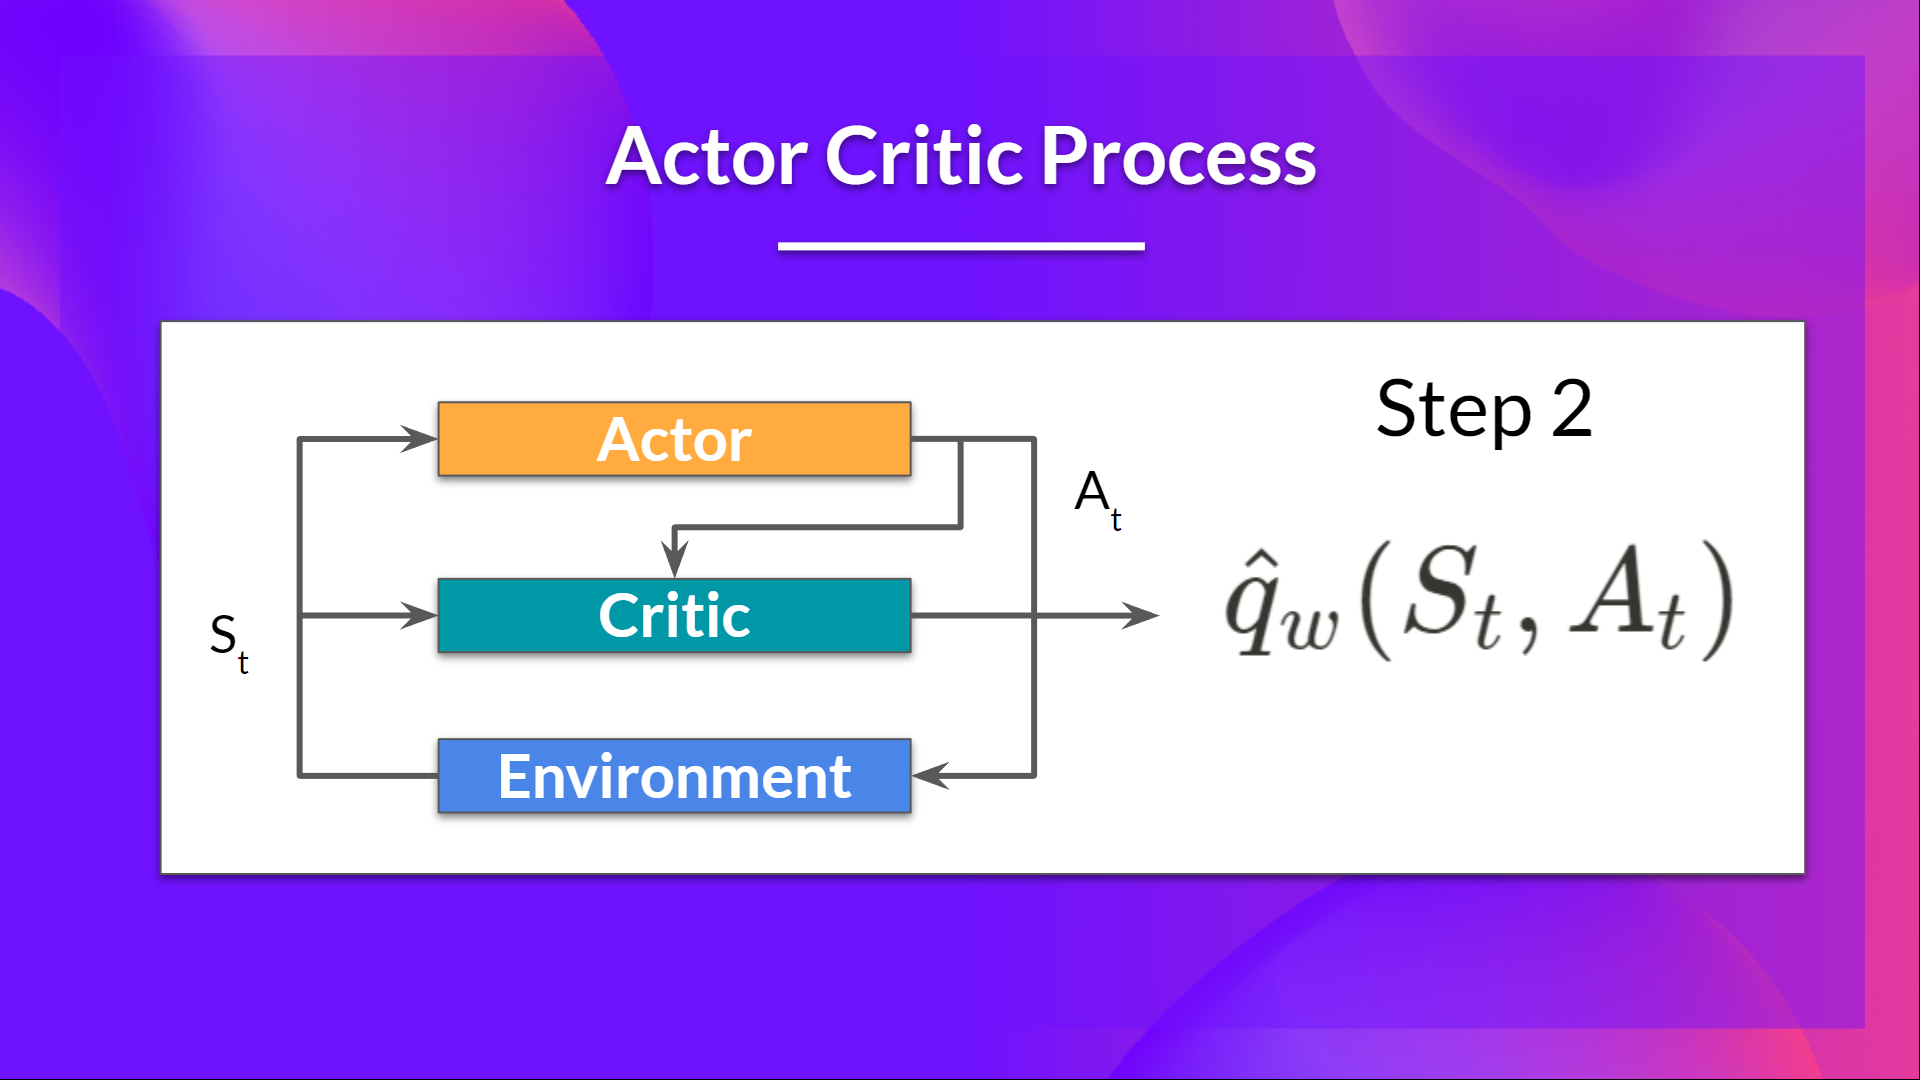
\includegraphics[width=0.6\linewidth,keepaspectratio]{rl141}
\end{center}
\end{frame}

%%%%%%%%%%%%%%%%%%%%%%%%%%%%%%%%%%%%%%%%%%%%%%%%%%%%%%%%%%%%%%%%%%%%%%%%%%%%%%%%%%
\begin{frame}[fragile]\frametitle{The Actor-Critic Process}

The action $A_t$ performed in the environment outputs a new state $S_{t+1}$ and a reward $R_{t+1}$
	
\begin{center}
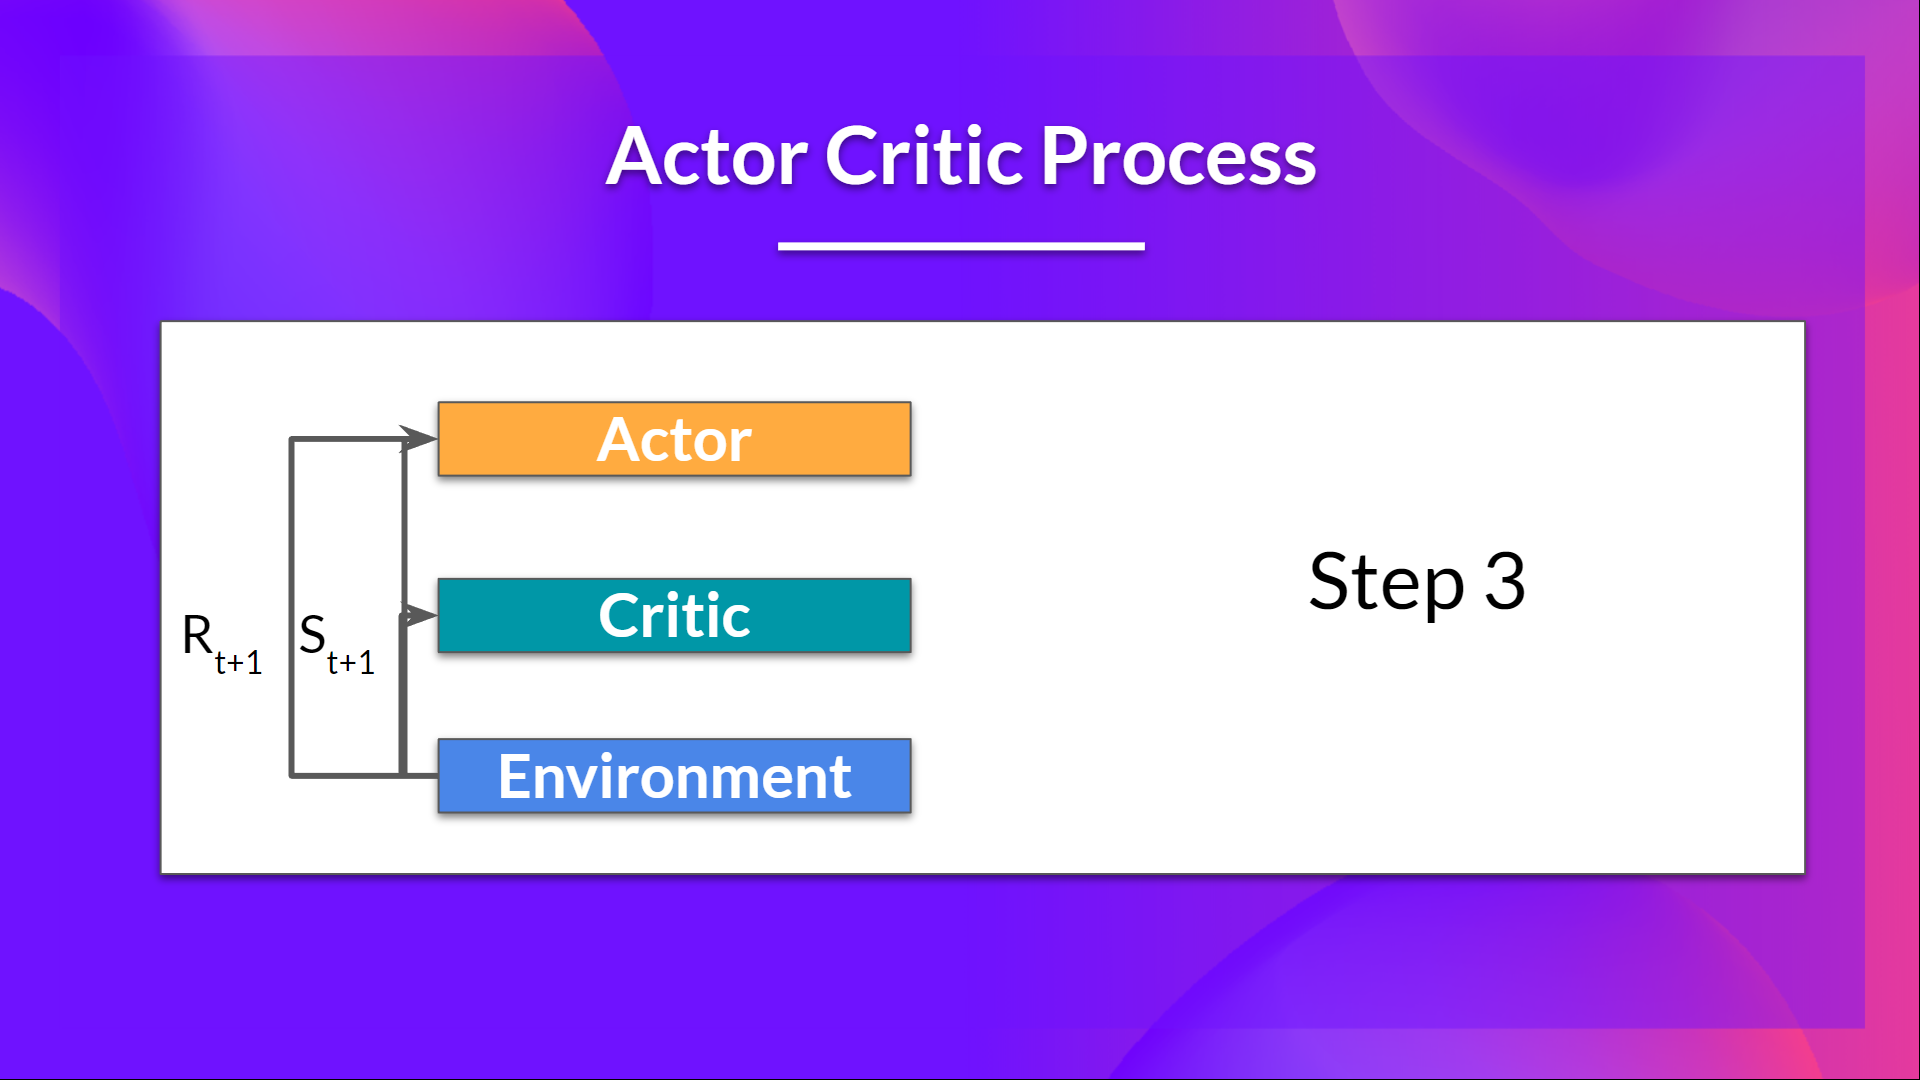
\includegraphics[width=0.6\linewidth,keepaspectratio]{rl142}
\end{center}
\end{frame}

%%%%%%%%%%%%%%%%%%%%%%%%%%%%%%%%%%%%%%%%%%%%%%%%%%%%%%%%%%%%%%%%%%%%%%%%%%%%%%%%%%
\begin{frame}[fragile]\frametitle{The Actor-Critic Process}

The Actor updates its policy parameters using the Q value.
	
\begin{center}
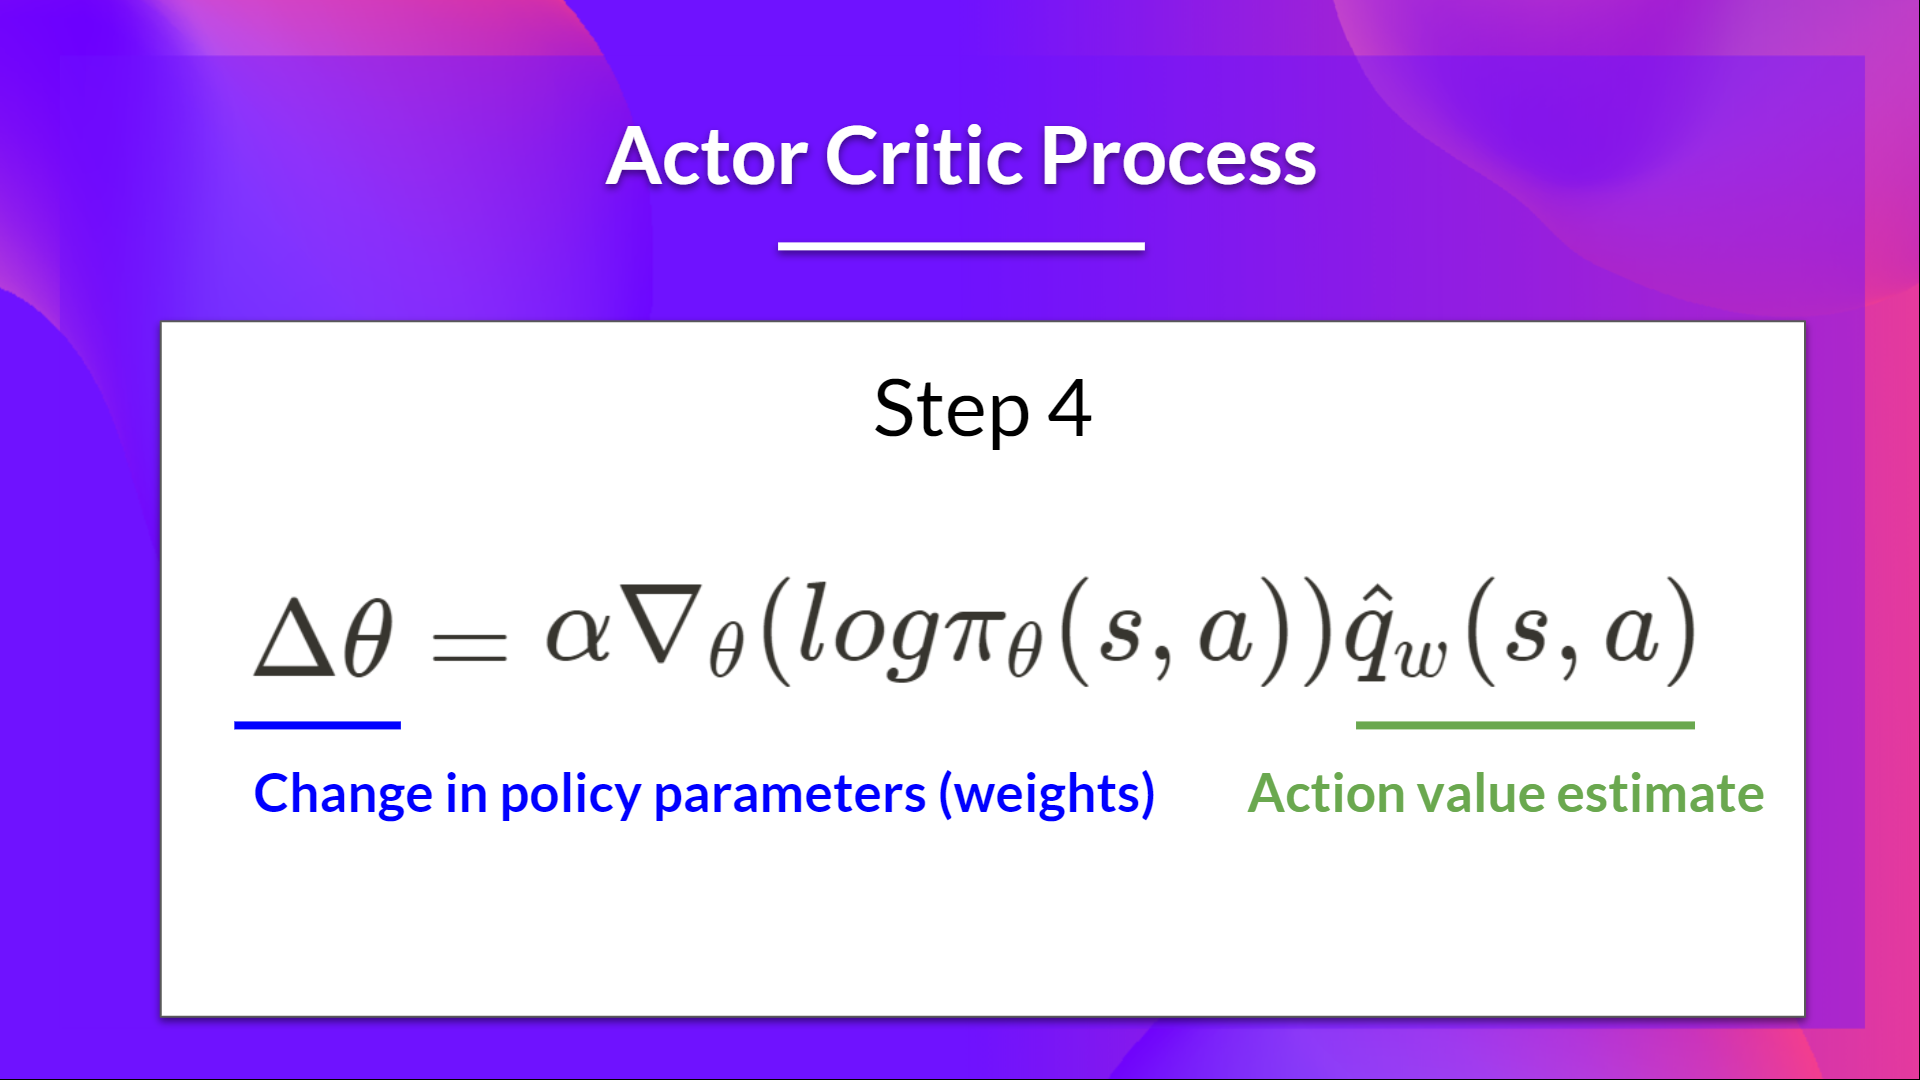
\includegraphics[width=0.6\linewidth,keepaspectratio]{rl143}
\end{center}
\end{frame}

%%%%%%%%%%%%%%%%%%%%%%%%%%%%%%%%%%%%%%%%%%%%%%%%%%%%%%%%%%%%%%%%%%%%%%%%%%%%%%%%%%
\begin{frame}[fragile]\frametitle{The Actor-Critic Process}

Thanks to its updated parameters, the Actor produces the next action to take at $A_{t+1}$  given the new state $S_{t+1}$. The Critic then updates its value parameters.	
\begin{center}
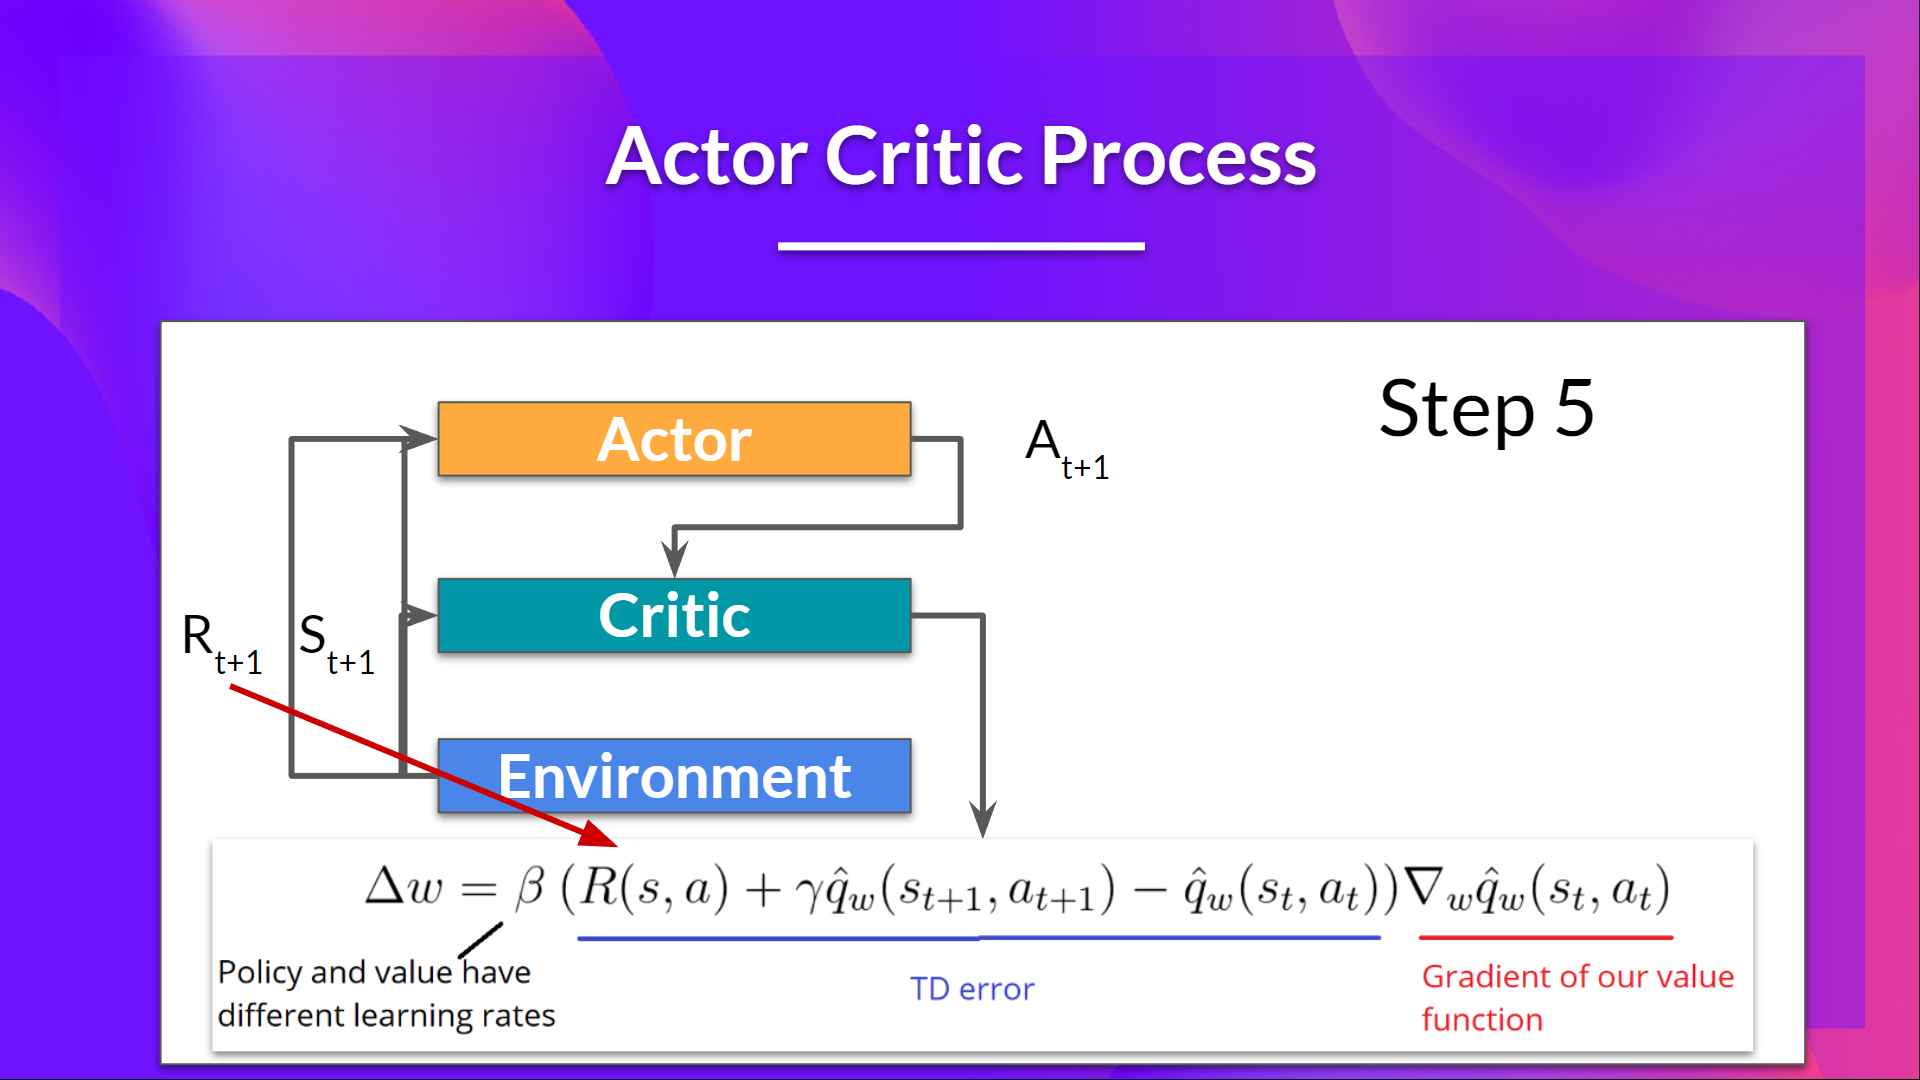
\includegraphics[width=0.6\linewidth,keepaspectratio]{rl144}
\end{center}
\end{frame}


%%%%%%%%%%%%%%%%%%%%%%%%%%%%%%%%%%%%%%%%%%%%%%%%%%%%%%%%%%%%%%%%%%%%%%%%%%%%%%%%%%
\begin{frame}[fragile]\frametitle{Advantage Actor Critic (A2C)}

\begin{itemize}
\item We can stabilize learning further by using the Advantage function as Critic instead of the Action value function.
\item The idea is that the Advantage function calculates how better taking that action at a state is compared to the average value of the state. It’s subtracting the mean value of the state from the state action pair:
\item In other words, this function calculates the extra reward we get if we take this action at that state compared to the mean reward we get at that state.
\end{itemize}


\begin{center}
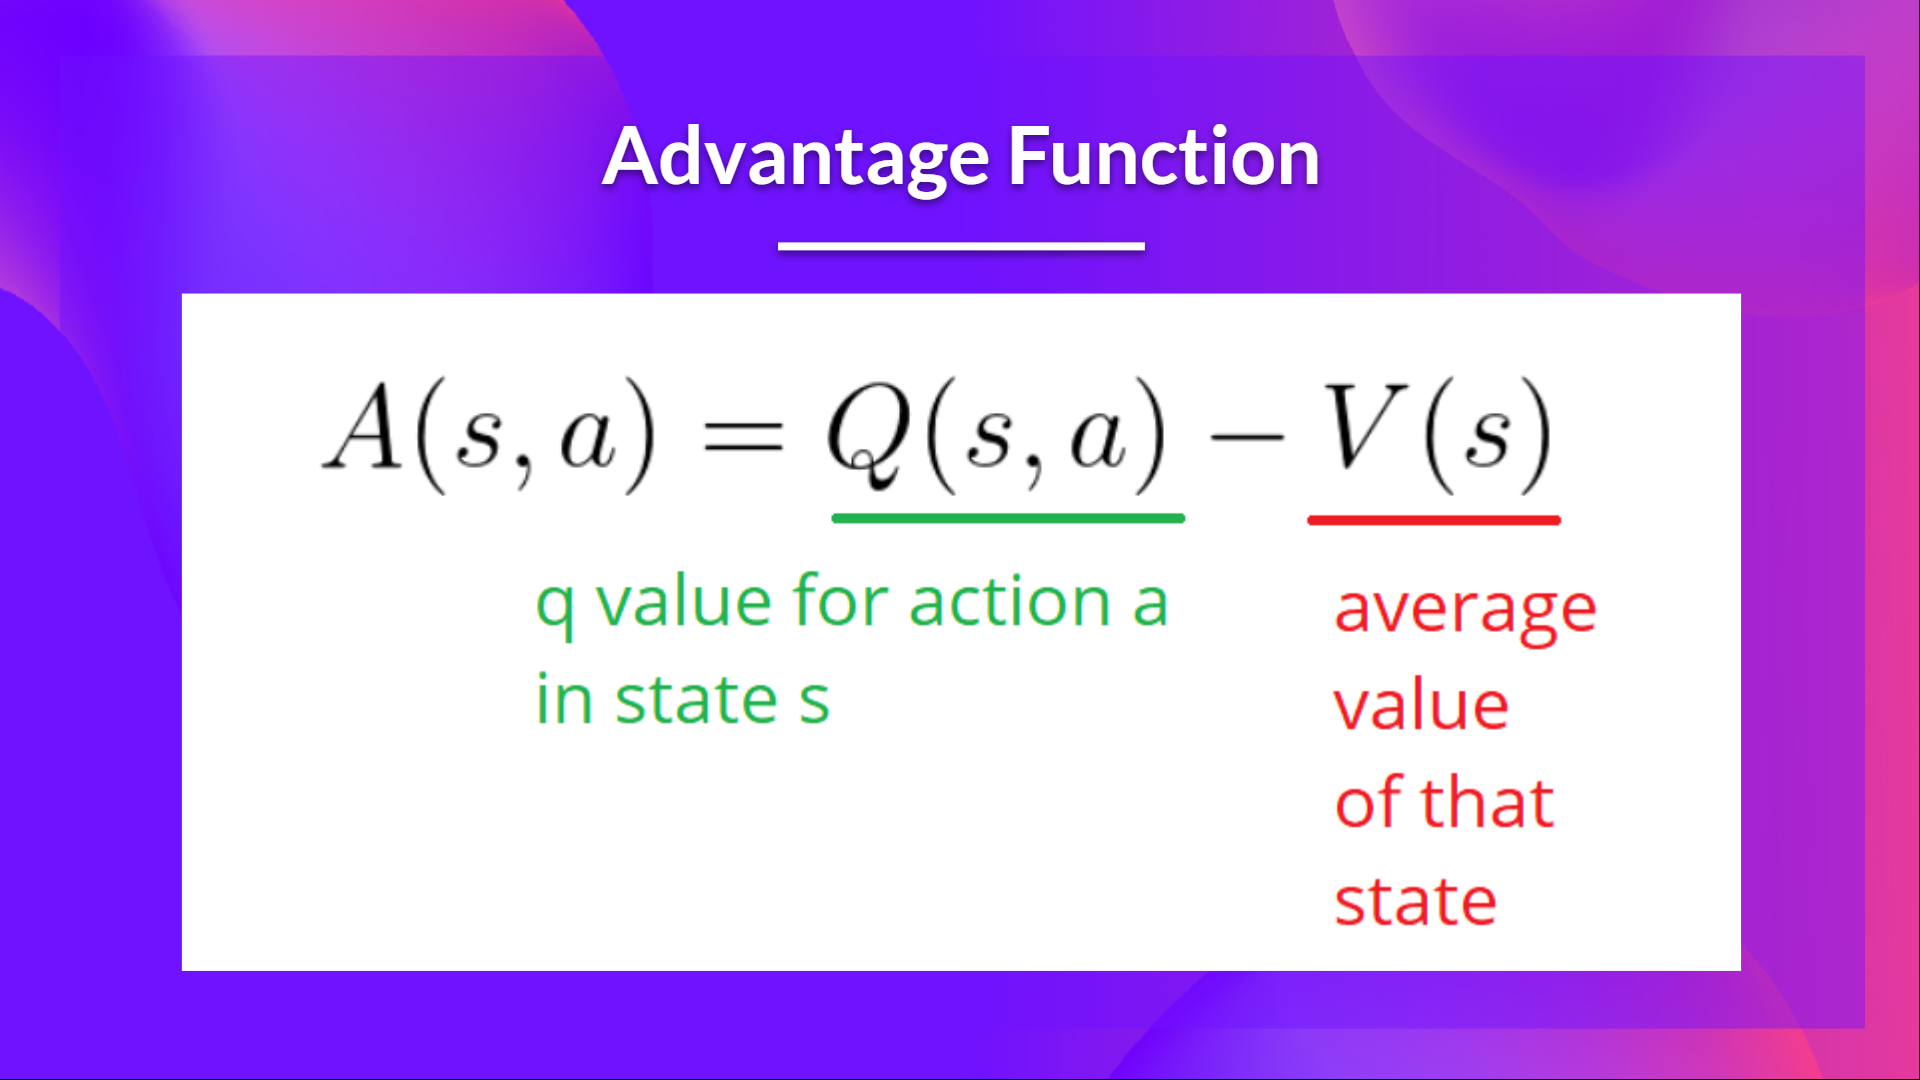
\includegraphics[width=0.6\linewidth,keepaspectratio]{rl145}
\end{center}



\end{frame}

%%%%%%%%%%%%%%%%%%%%%%%%%%%%%%%%%%%%%%%%%%%%%%%%%%%%%%%%%%%%%%%%%%%%%%%%%%%%%%%%%%
\begin{frame}[fragile]\frametitle{Advantage Actor Critic (A2C)}

The problem with implementing this advantage function is that it requires two value functions — $Q(s,a)$ and $V(s)$. Fortunately, we can use the TD error as a good estimator of the advantage function.

\begin{center}
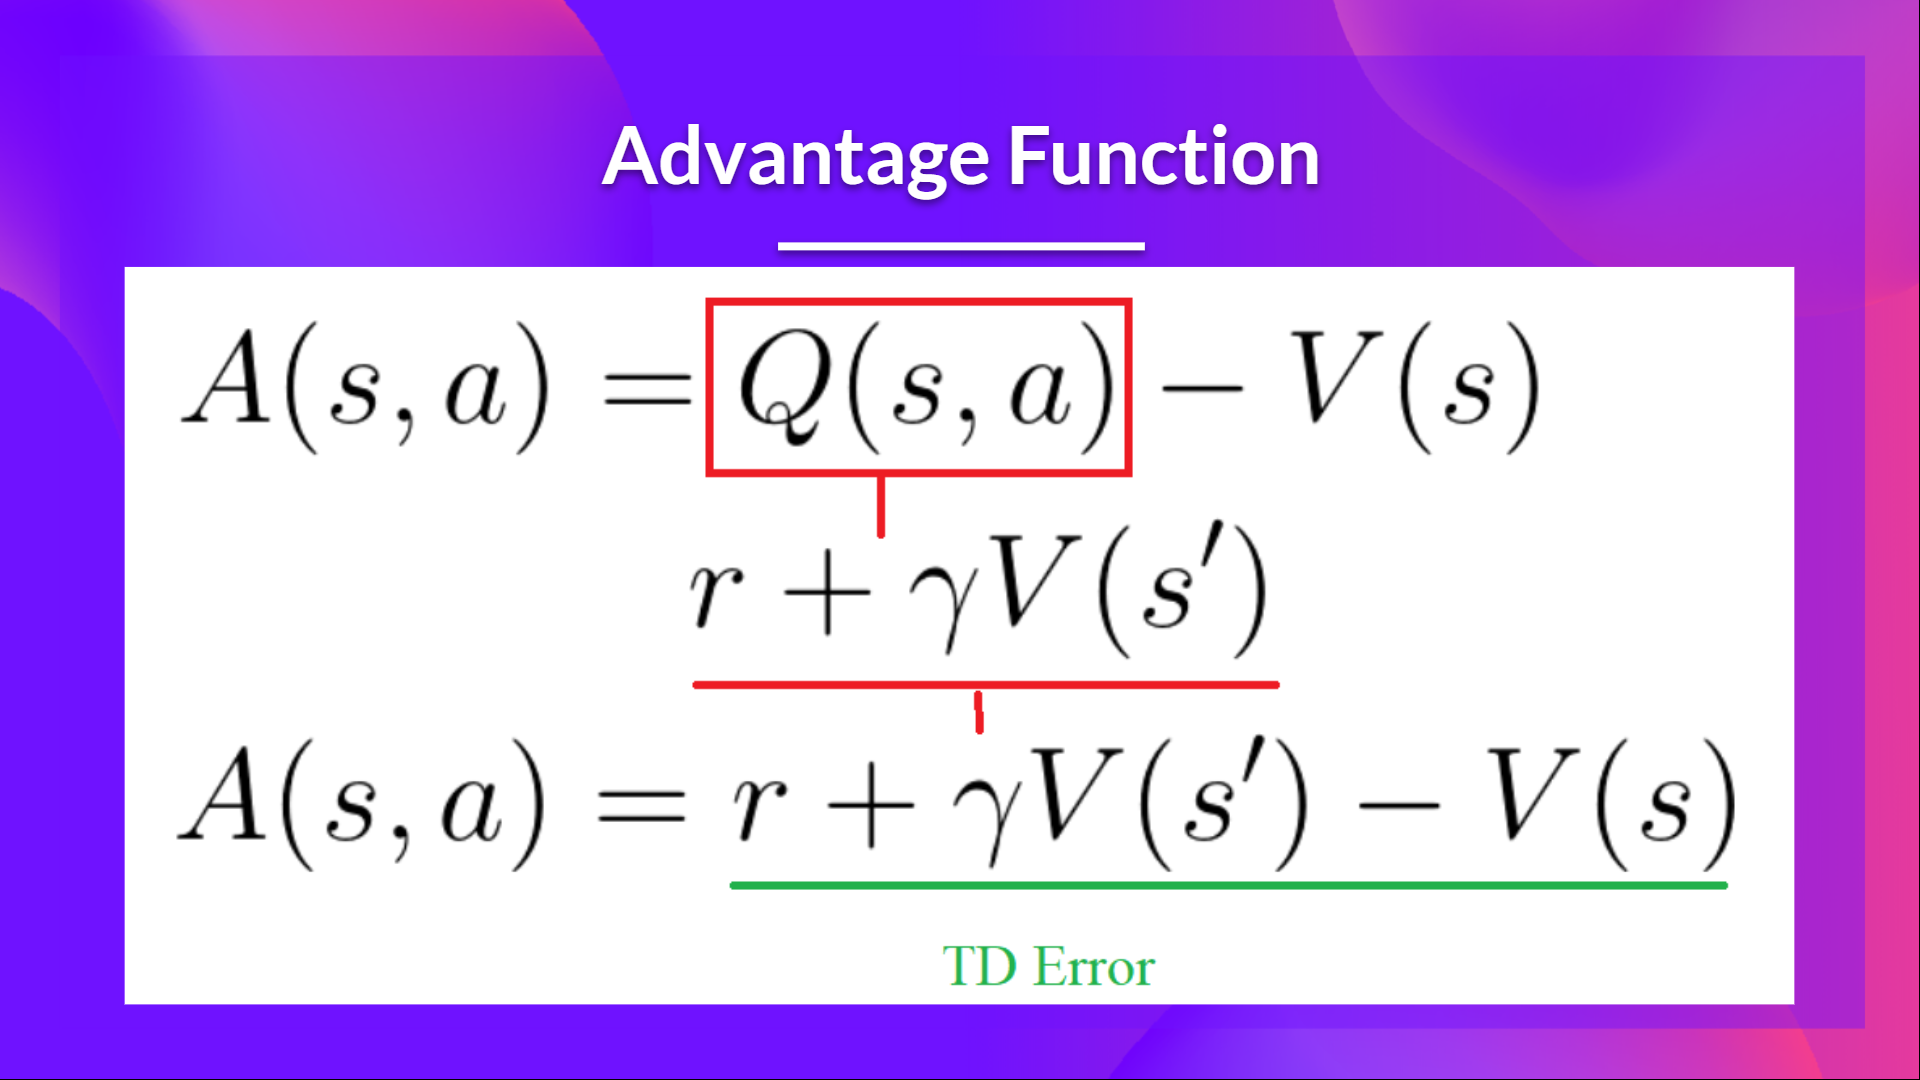
\includegraphics[width=0.6\linewidth,keepaspectratio]{rl146}
\end{center}


\end{frame}


%%%%%%%%%%%%%%%%%%%%%%%%%%%%%%%%%%%%%%%%%%%%%%%%%%%%%%%%%%%%%%%%%%%%%%%%%%%%%%%%%%
\begin{frame}[fragile]\frametitle{Advantage Actor Critic (A2C)}

The extra reward is what's beyond the expected value of that state.

\begin{itemize}
\item If $A(s,a) > 0$: our gradient is pushed in that direction.
\item If $A(s,a) < 0$ (our action does worse than the average value of that state), our gradient is pushed in the opposite direction.
\end{itemize}

\end{frame}

%%%%%%%%%%%%%%%%%%%%%%%%%%%%%%%%%%%%%%%%%%%%%%%%%%%%%%%%%%%%%%%%%%%%%%%%%%%%%%%%%%
\begin{frame}[fragile]\frametitle{}
\begin{center}
{\Large Proximal Policy Optimization (PPO)}
\end{center}

{\tiny (Ref: Proximal Policy Optimization (PPO) https://huggingface.co/blog/deep-rl-ppo)}

\end{frame}

%%%%%%%%%%%%%%%%%%%%%%%%%%%%%%%%%%%%%%%%%%%%%%%%%%%%%%%%%%%%%%%%%%%%%%%%%%%%%%%%%%
\begin{frame}[fragile]\frametitle{The intuition behind PPO}

To improve the training stability of the policy by limiting the change you make to the policy at each training epoch: to avoid having too large policy updates. For two reasons:

\begin{itemize}
\item We know empirically that smaller policy updates during training are more likely to converge to an optimal solution.
\item A too big step in a policy update can result in falling “off the cliff” (getting a bad policy) and having a long time or even no possibility to recover.
\item So with PPO, we update the policy conservatively. To do so, we need to measure how much the current policy changed compared to the former one using a ratio calculation between the current and former policy. 
\item And we clip this ratio in a range $[1 - \epsilon, 1 + \epsilon]$, meaning that we remove the incentive for the current policy to go too far from the old one (hence the proximal policy term).
\end{itemize}

\end{frame}

%%%%%%%%%%%%%%%%%%%%%%%%%%%%%%%%%%%%%%%%%%%%%%%%%%%%%%%%%%%%%%%%%%%%%%%%%%%%%%%%%%
\begin{frame}[fragile]\frametitle{Recap: The Policy Objective Function}

\begin{center}
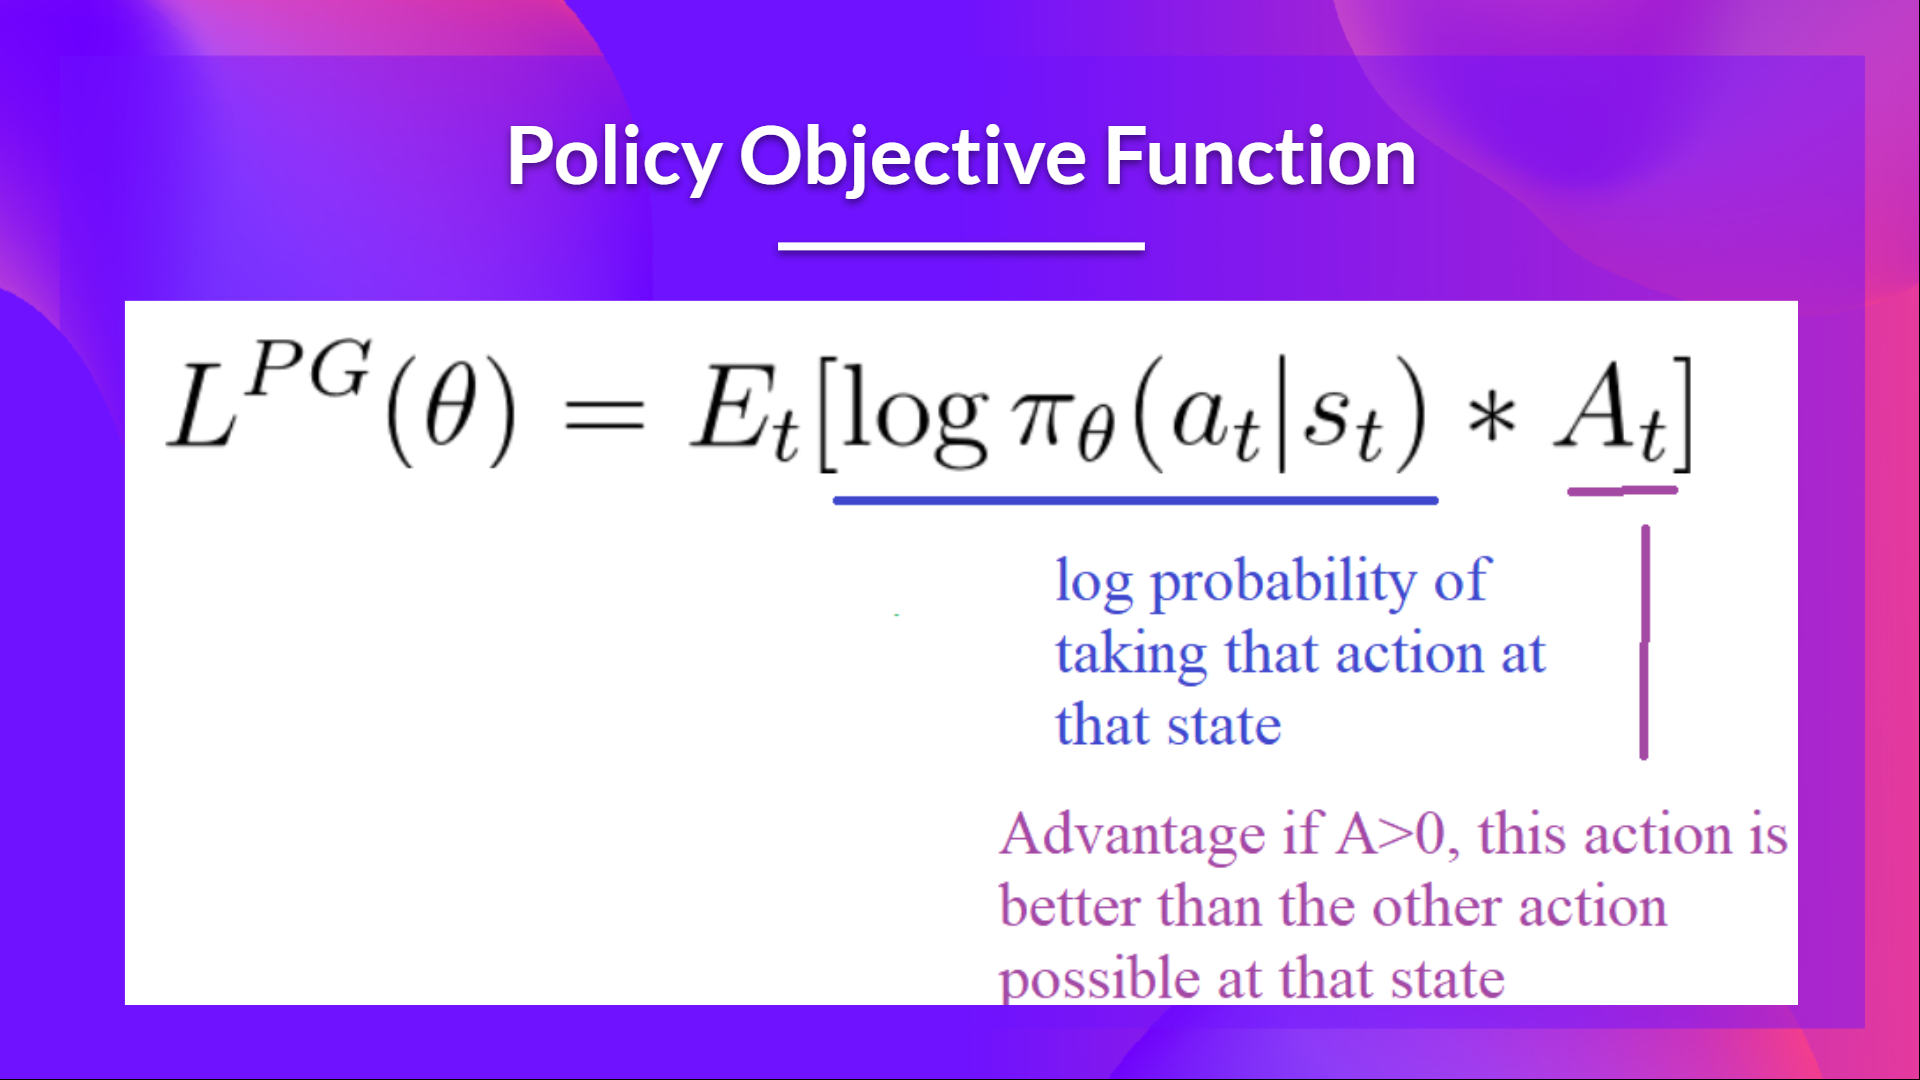
\includegraphics[width=0.6\linewidth,keepaspectratio]{rl147}
\end{center}

The idea was that by taking a gradient ascent step on this function (equivalent to taking gradient descent of the negative of this function), we would push our agent to take actions that lead to higher rewards and avoid harmful actions.

\end{frame}

%%%%%%%%%%%%%%%%%%%%%%%%%%%%%%%%%%%%%%%%%%%%%%%%%%%%%%%%%%%%%%%%%%%%%%%%%%%%%%%%%%
\begin{frame}[fragile]\frametitle{Recap: The Policy Objective Function}

However, the problem comes from the step size:

\begin{itemize}
\item Too small, the training process was too slow
\item Too high, there was too much variability in the training
\end{itemize}

Here with PPO, the idea is to constrain our policy update with a new objective function called the Clipped surrogate objective function that will constrain the policy change in a small range using a clip.

\end{frame}


%%%%%%%%%%%%%%%%%%%%%%%%%%%%%%%%%%%%%%%%%%%%%%%%%%%%%%%%%%%%%%%%%%%%%%%%%%%%%%%%%%
\begin{frame}[fragile]\frametitle{Recap: The Policy Objective Function}

This new function is designed to avoid destructive large weights updates :

\begin{center}
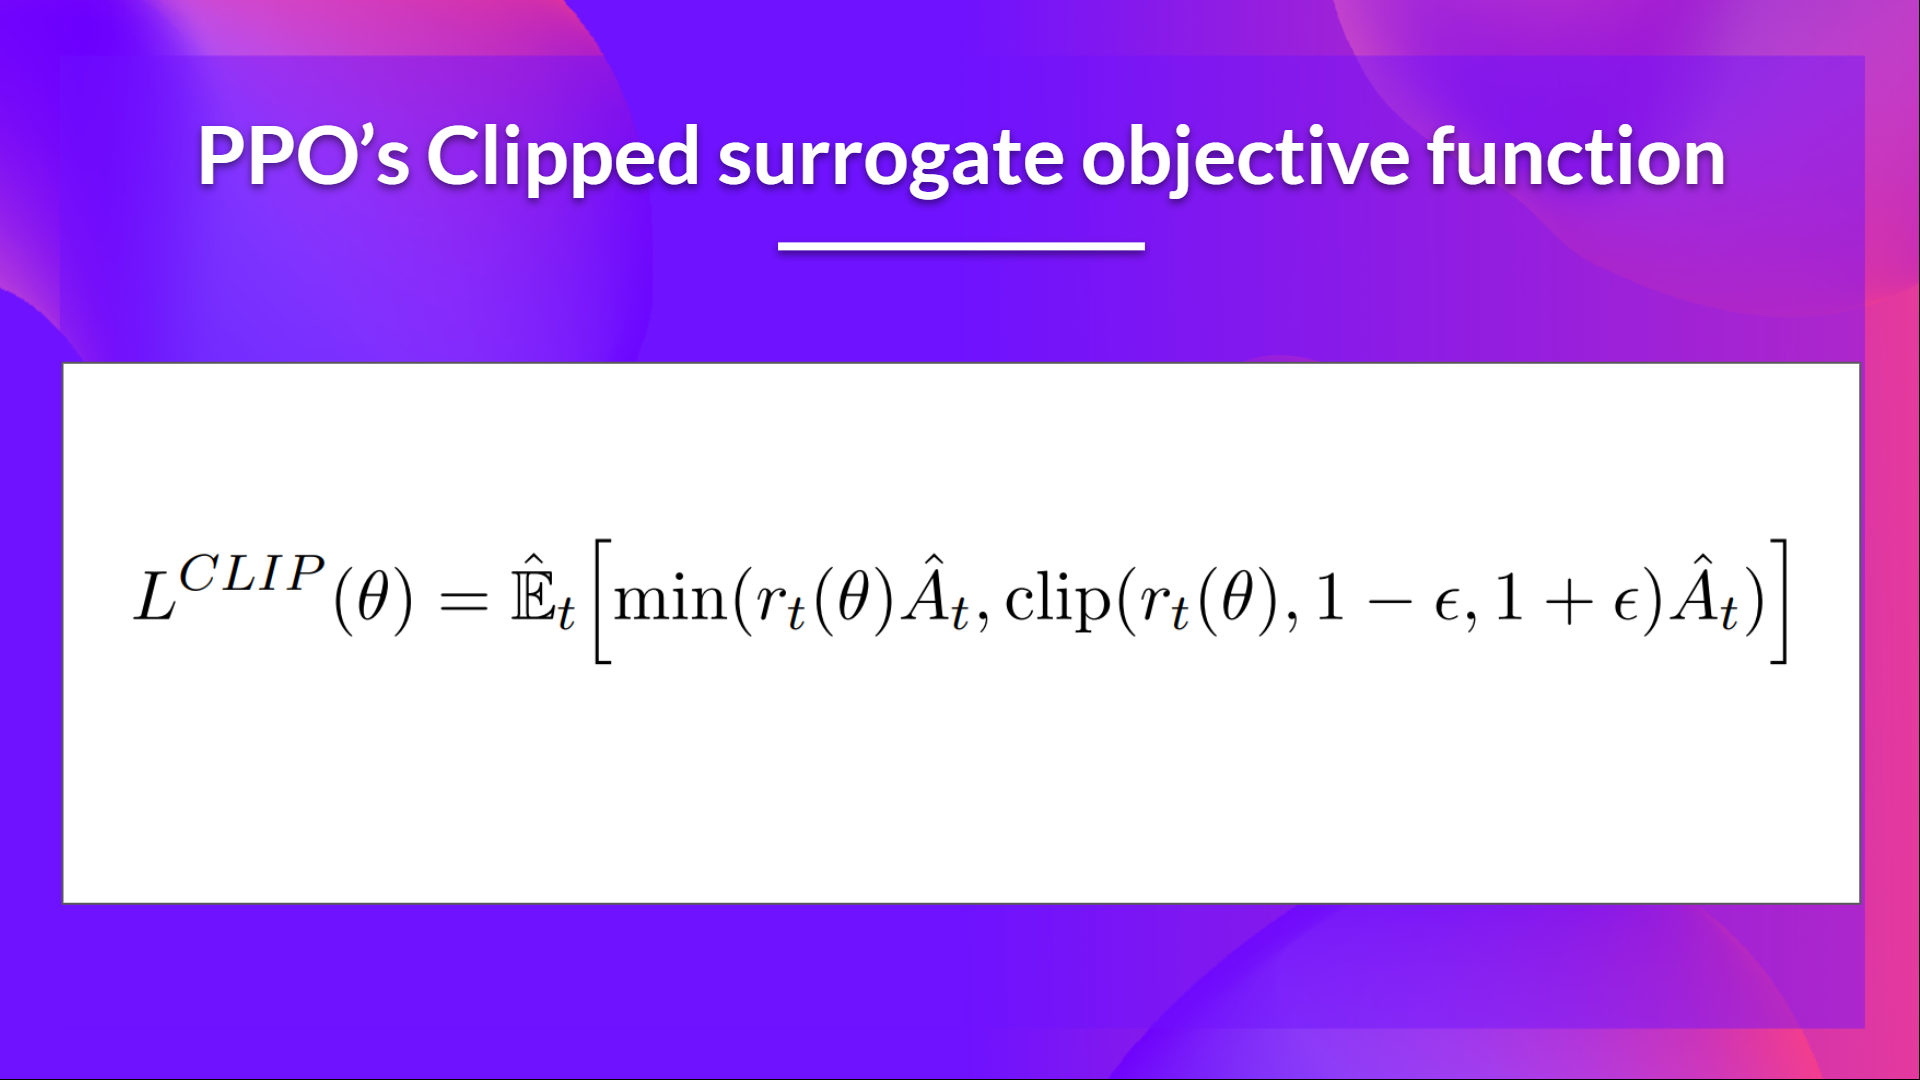
\includegraphics[width=0.6\linewidth,keepaspectratio]{rl148}
\end{center}

\end{frame}

%%%%%%%%%%%%%%%%%%%%%%%%%%%%%%%%%%%%%%%%%%%%%%%%%%%%%%%%%%%%%%%%%%%%%%%%%%%%%%%%%%
\begin{frame}[fragile]\frametitle{The Ratio Function}

This new function is designed to avoid destructive large weights updates :

\begin{center}
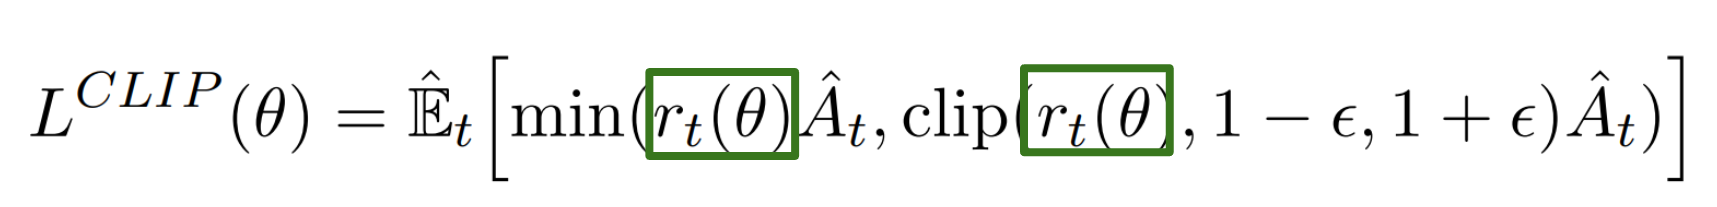
\includegraphics[width=0.8\linewidth,keepaspectratio]{rl149}
\end{center}



This ratio is calculated this way:

\begin{center}
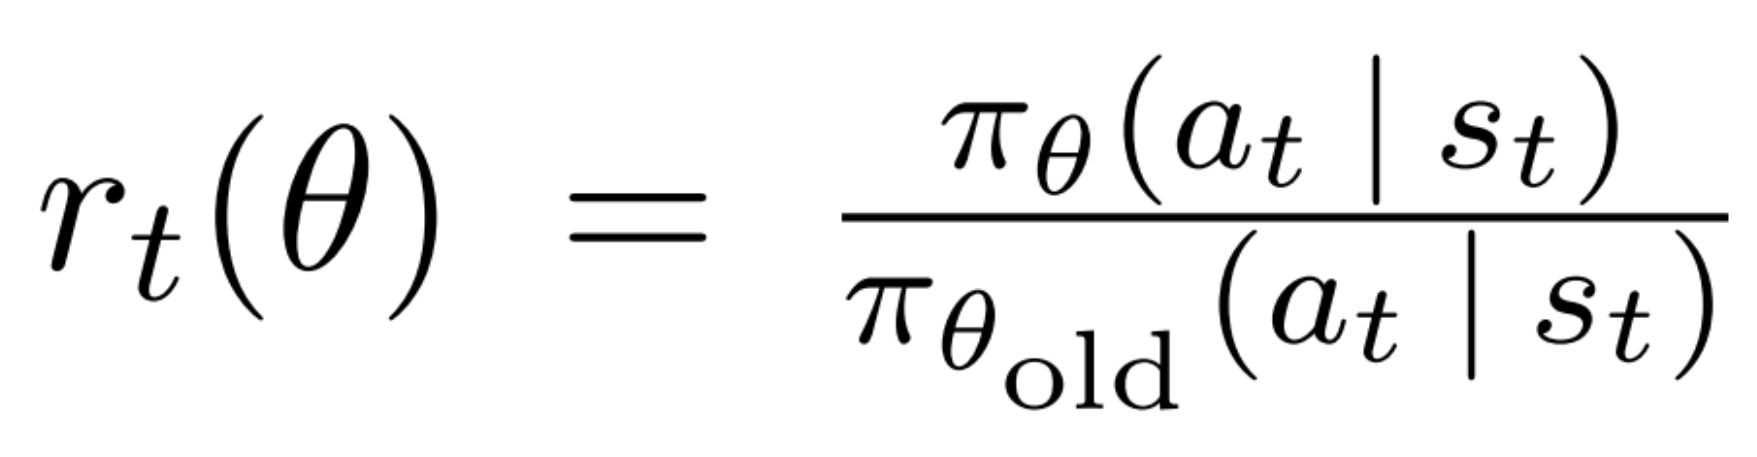
\includegraphics[width=0.4\linewidth,keepaspectratio]{rl150}
\end{center}

It’s the probability of taking action $a_t$ at state $s_t$ in the current policy divided by the previous one.

\end{frame}


%%%%%%%%%%%%%%%%%%%%%%%%%%%%%%%%%%%%%%%%%%%%%%%%%%%%%%%%%%%%%%%%%%%%%%%%%%%%%%%%%%
\begin{frame}[fragile]\frametitle{Recap: The Policy Objective Function}

As we can see, $r_t(\theta)$ denotes the probability ratio between the current and old policy:

\begin{itemize}
\item If $r_t(\theta) > 0$ the action $a_t$ at state $s_t$ is more likely in the current policy than the old policy.
\item If $r_t(\theta)$ is between 0 and 1, the action is less likely for the current policy than for the old one.
\end{itemize}

So this probability ratio is an easy way to estimate the divergence between old and current policy.

\end{frame}

%%%%%%%%%%%%%%%%%%%%%%%%%%%%%%%%%%%%%%%%%%%%%%%%%%%%%%%%%%%%%%%%%%%%%%%%%%%%%%%%%%
\begin{frame}[fragile]\frametitle{The unclipped part of the Clipped Surrogate Objective function}

\begin{center}
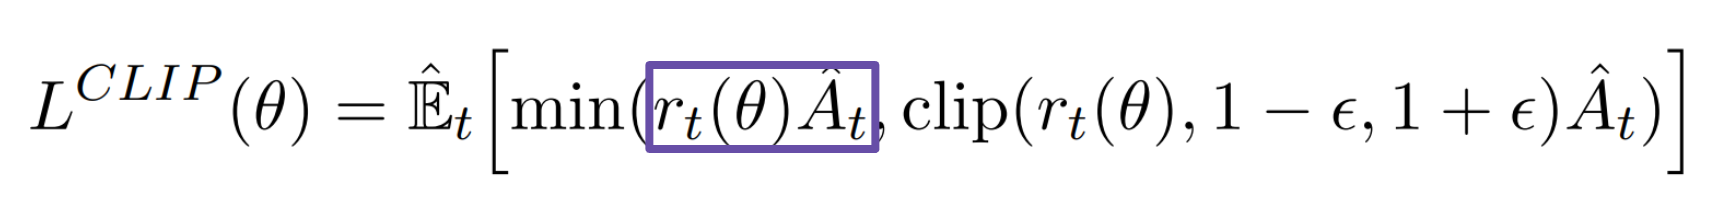
\includegraphics[width=0.8\linewidth,keepaspectratio]{rl151}
\end{center}


This ratio can replace the log probability we use in the policy objective function. This gives us the left part of the new objective function: multiplying the ratio by the advantage

\begin{center}
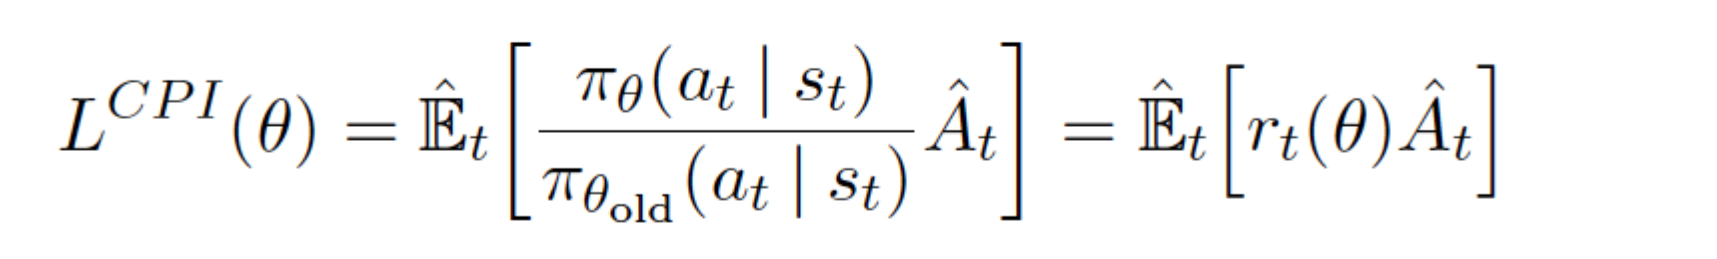
\includegraphics[width=0.8\linewidth,keepaspectratio]{rl152}
\end{center}

However, without a constraint, if the action taken is much more probable in our current policy than in our former, this would lead to a significant policy gradient step and, therefore, an excessive policy update.
\end{frame}

%%%%%%%%%%%%%%%%%%%%%%%%%%%%%%%%%%%%%%%%%%%%%%%%%%%%%%%%%%%%%%%%%%%%%%%%%%%%%%%%%%
\begin{frame}[fragile]\frametitle{The clipped Part of the Clipped Surrogate Objective function}

\begin{center}
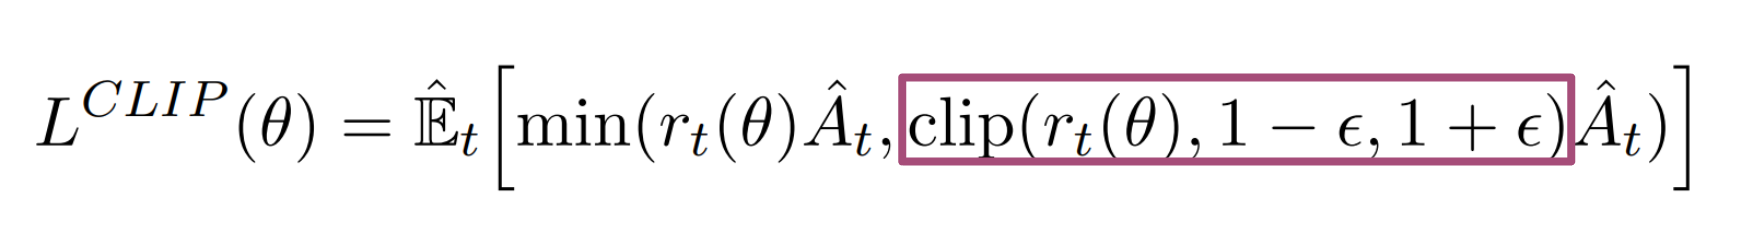
\includegraphics[width=0.8\linewidth,keepaspectratio]{rl153}
\end{center}


Consequently, we need to constrain this objective function by penalizing changes that lead to a ratio away from 1 (in the paper, the ratio can only vary from 0.8 to 1.2).
\end{frame}


%%%%%%%%%%%%%%%%%%%%%%%%%%%%%%%%%%%%%%%%%%%%%%%%%%%%%%%%%%%%%%%%%%%%%%%%%%%%%%%%%%
\begin{frame}[fragile]\frametitle{The clipped Part of the Clipped Surrogate Objective function}

By clipping the ratio, we ensure that we do not have a too large policy update because the current policy can't be too different from the older one.

To do that, we have two solutions:

\begin{itemize}
\item TRPO (Trust Region Policy Optimization) uses KL divergence constraints outside the objective function to constrain the policy update. But this method is complicated to implement and takes more computation time.
\item PPO clip probability ratio directly in the objective function with its Clipped surrogate objective function.
\end{itemize}


\end{frame}

%%%%%%%%%%%%%%%%%%%%%%%%%%%%%%%%%%%%%%%%%%%%%%%%%%%%%%%%%%%%%%%%%%%%%%%%%%%%%%%%%%
\begin{frame}[fragile]\frametitle{The clipped Part of the Clipped Surrogate Objective function}

\begin{center}
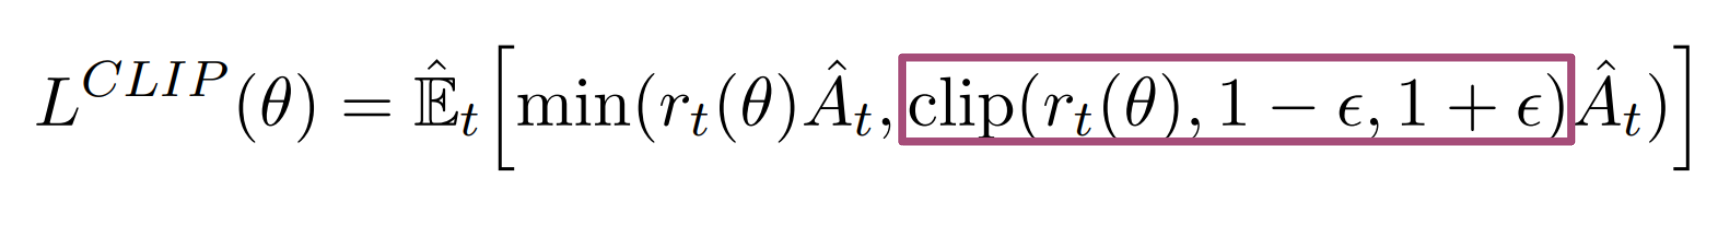
\includegraphics[width=0.8\linewidth,keepaspectratio]{rl154}
\end{center}


This clipped part is a version where rt(theta) is clipped between $[1 - \epsilon, 1 + \epsilon]$.
\end{frame}

%%%%%%%%%%%%%%%%%%%%%%%%%%%%%%%%%%%%%%%%%%%%%%%%%%%%%%%%%%%%%%%%%%%%%%%%%%%%%%%%%%
\begin{frame}[fragile]\frametitle{The clipped Part of the Clipped Surrogate Objective function}

\begin{itemize}
\item With the Clipped Surrogate Objective function, we have two probability ratios, one non-clipped and one clipped in a range (between $[1 - \epsilon, 1 + \epsilon]$, epsilon is a hyperparameter that helps us to define this clip range (in the paper $\epsilon = 0.2$).

\item Then, we take the minimum of the clipped and non-clipped objective, so the final objective is a lower bound (pessimistic bound) of the unclipped objective.

\item Taking the minimum of the clipped and non-clipped objective means we'll select either the clipped or the non-clipped objective based on the ratio and advantage situation.
\end{itemize}


\end{frame}


%%%%%%%%%%%%%%%%%%%%%%%%%%%%%%%%%%%%%%%%%%%%%%%%%%%%%%%%%%%%%%%%%%%%%%%%%%%%%%%%%%
\begin{frame}[fragile]\frametitle{Visualize the Clipped Surrogate Objective}

\begin{center}
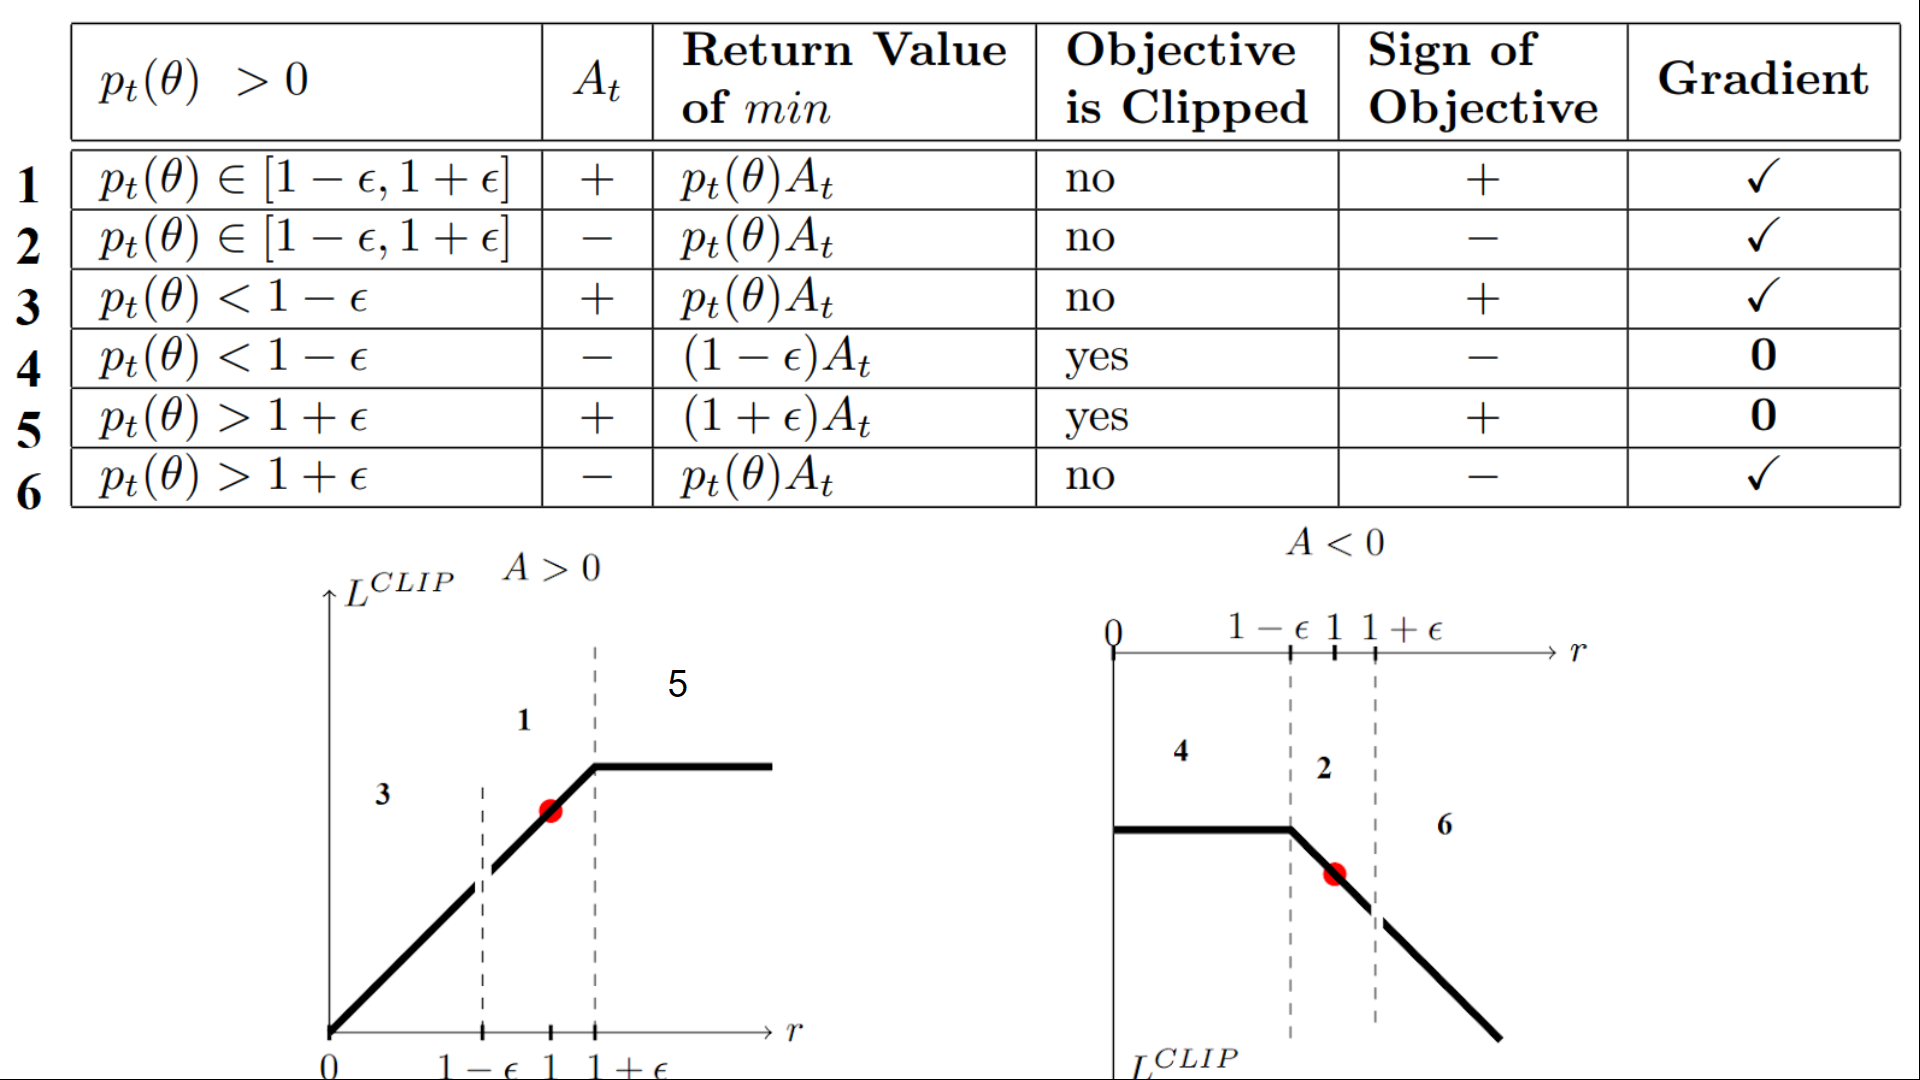
\includegraphics[width=0.8\linewidth,keepaspectratio]{rl155}

{\tiny (Ref: Table from "Towards Delivering a Coherent Self-Contained Explanation of Proximal Policy Optimization" by Daniel Bick)}

\end{center}


We have six different situations. Remember first that we take the minimum between the clipped and unclipped objectives.
\end{frame}


%%%%%%%%%%%%%%%%%%%%%%%%%%%%%%%%%%%%%%%%%%%%%%%%%%%%%%%%%%%%%%%%%%%%%%%%%%%%%%%%%%
\begin{frame}[fragile]\frametitle{Case 1 and 2: the ratio is between the range}

\begin{itemize}
\item In situations 1 and 2, the clipping does not apply since the ratio is between the range $[1 - \epsilon, 1 + \epsilon]$
\item In situation 1, we have a positive advantage: the action is better than the average of all the actions in that state. Therefore, we should encourage our current policy to increase the probability of taking that action in that state.
\item Since the ratio is between intervals, we can increase our policy's probability of taking that action at that state.
\item In situation 2, we have a negative advantage: the action is worse than the average of all actions at that state. Therefore, we should discourage our current policy from taking that action in that state.
\item Since the ratio is between intervals, we can decrease the probability that our policy takes that action at that state.
\end{itemize}


\end{frame}

%%%%%%%%%%%%%%%%%%%%%%%%%%%%%%%%%%%%%%%%%%%%%%%%%%%%%%%%%%%%%%%%%%%%%%%%%%%%%%%%%%
\begin{frame}[fragile]\frametitle{Case 3 and 4: the ratio is below the range}

\begin{itemize}
\item If the probability ratio is lower than $[1 - \epsilon]$, the probability of taking that action at that state is much lower than with the old policy.
\item If, like in situation 3, the advantage estimate is positive $(A>0)$, then you want to increase the probability of taking that action at that state.
\item 
But if, like situation 4, the advantage estimate is negative, we don't want to decrease further the probability of taking that action at that state. Therefore, the gradient is = 0 (since we're on a flat line), so we don't update our weights.
\end{itemize}


\end{frame}

%%%%%%%%%%%%%%%%%%%%%%%%%%%%%%%%%%%%%%%%%%%%%%%%%%%%%%%%%%%%%%%%%%%%%%%%%%%%%%%%%%
\begin{frame}[fragile]\frametitle{Case 5 and 6: the ratio is above the range}

\begin{itemize}
\item If the probability ratio is higher than $[1 + \epsilon]$, the probability of taking that action at that state in the current policy is much higher than in the former policy.
\item 
If, like in situation 5, the advantage is positive, we don't want to get too greedy. We already have a higher probability of taking that action at that state than the former policy. Therefore, the gradient is = 0 (since we're on a flat line), so we don't update our weights.
\item 
If, like in situation 6, the advantage is negative, we want to decrease the probability of taking that action at that state.
\end{itemize}
\end{frame}

%%%%%%%%%%%%%%%%%%%%%%%%%%%%%%%%%%%%%%%%%%%%%%%%%%%%%%%%%%%%%%%%%%%%%%%%%%%%%%%%%%
\begin{frame}[fragile]\frametitle{Conclusion}
So if we recap, we only update the policy with the unclipped objective part. When the minimum is the clipped objective part, we don't update our policy weights since the gradient will equal 0. So we update our policy only if:

\begin{itemize}
\item Our ratio is in the range $[1 - \epsilon, 1 + \epsilon]$
\item Our ratio is outside the range, but the advantage leads to getting closer to the range
\begin{itemize}
\item Being below the ratio but the advantage is $> 0$
\item Being above the ratio but the advantage is $< 0$
\end{itemize}

\item You might wonder why, when the minimum is the clipped ratio, the gradient is 0. When the ratio is clipped, the derivative in this case will not be the derivative of the $r_t(\theta) * A_t$ but the derivative of either $(1 - \epsilon)* A_t$  or the derivative of $(1 + \epsilon)* A_t$  which both = 0.
\end{itemize}
\end{frame}

%%%%%%%%%%%%%%%%%%%%%%%%%%%%%%%%%%%%%%%%%%%%%%%%%%%%%%%%%%%%%%%%%%%%%%%%%%%%%%%%%%
\begin{frame}[fragile]\frametitle{Conclusion}

\begin{itemize}
\item To summarize, thanks to this clipped surrogate objective, we restrict the range that the current policy can vary from the old one. Because we remove the incentive for the probability ratio to move outside of the interval since, the clip have the effect to gradient. If the ratio is $> 1 + \epsilon$ or $< 1 - \epsilon$ the gradient will be equal to 0.

\item  The final Clipped Surrogate Objective Loss for PPO Actor-Critic style looks like this, it's a combination of Clipped Surrogate Objective function, Value Loss Function and Entropy bonus
\end{itemize}

\begin{center}
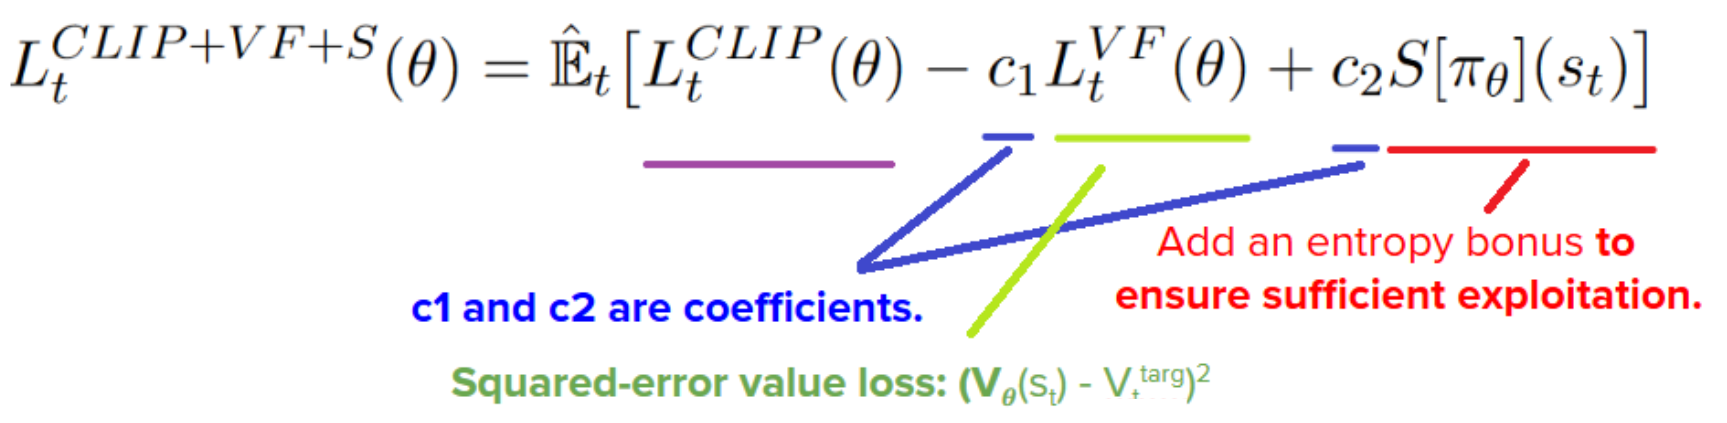
\includegraphics[width=0.8\linewidth,keepaspectratio]{rl156}
\end{center}
\end{frame}